% Compile with XeLaTeX:  latexmk -xelatex main.tex
\documentclass[11pt,a4paper]{article}
\usepackage{fontspec}
\setmainfont{FreeSerif}
\setsansfont{FreeSans}
\setmonofont[Scale=0.86]{DejaVu Sans Mono}
\usepackage{amsmath,amssymb}
\usepackage[margin=2.4cm]{geometry}
\usepackage{graphicx}
\usepackage{booktabs,longtable,array}
\usepackage{enumitem}
\usepackage{xcolor}
\usepackage{caption}
\usepackage[hidelinks]{hyperref}
\usepackage{microtype}
\captionsetup{font=small,labelfont=bf}
\setlist{nosep}
\graphicspath{{figures/}}
\newcommand{\nGraphSteps}{12}
\newcommand{\nSteps}{13}
\newcommand{\nNodes}{78}
\newcommand{\nStateNodes}{23}
\newcommand{\nModelNodes}{21}
\newcommand{\nObsNodes}{34}
\newcommand{\nRefs}{87}
\newcommand{\nFinalSectors}{10}
\newcommand{\nFinalClusters}{6}
\newcommand{\nFinalFund}{7}
\newcommand{\nFinalAbsorbed}{3}
\newcommand{\nFinalRoutes}{12}
\newcommand{\nFinalObs}{16}
\newcommand{\nFinalUnexplained}{1}
\newcommand{\nFinalEdges}{22}
\newcommand{\maxEffective}{2}
\newcommand{\nFinalFit}{4}
\newcommand{\nAnomalySteps}{6}
\newcommand{\nPredSteps}{2}

\newcommand{\gen}{Great Epistemic Network}
\newcommand{\live}{\url{https://tahmeedhossain.github.io/GEN_HEP/}}
\newcommand{\repo}{\url{https://github.com/tahmeedhossain/GEN_HEP}}
\newcommand{\lay}[1]{\textsf{#1}}
\newcommand{\id}[1]{\texttt{#1}}

\title{A growing concept graph of particle physics:\\states, models and observables from one-particle quantum mechanics to the electroweak Standard Model}
\author{Tahmeed Hossain\\[2pt]\small Department of Theoretical Physics, University of Dhaka}
\date{\small 12 November 2026 (v1.2) \\[4pt] \small Graph data, interactive page and this text are generated with an AI assistant (Claude, Anthropic) under the author's direction; see Section~\ref{sec:ai}.}

\begin{document}
\maketitle

\begin{abstract}
We represent the development of particle physics, from one-particle quantum mechanics (1925) to the electroweak Standard Model with its Higgs sector (2012), as a concept graph with three layers: \emph{states} (what the theory says can exist), \emph{models} (the postulates and Lagrangian terms that act on states) and \emph{observables} (what is measured). Edges name the mathematical connection between two nodes, and interaction terms are entered by AND routes from the occupation-number nodes of several field sectors. The graph is built in \nGraphSteps{} steps that follow the historical and logical order: the state layer is partitioned into Wigner's irreducible representations, an unexplained observable (creation and destruction of particles) forces a field node that extends each representation into a Fock ladder, effective interaction nodes (QED vertex, Fermi and muon-decay contact terms, V$-$A) are added as they were discovered and then merged into the fundamental vertices of SU(2)$_L\times$U(1)$_Y$ and the Higgs sector, and the final step clusters every vertex inside the Lagrangian term it belongs to, with the effective nodes absorbed in the term that reproduces them at low energy. From the sequence we read off ten rules that govern how the graph grows (symmetry partition, in-degree-zero drive, Fock extension, route composition, universality merge, absorption, sector refinement, calibration, clustering, and the anomaly/prediction cycle), state them in graph terms, and check each against the step in which it fires. The interactive page, the data (\nNodes{} nodes, \nRefs{} references) and the scripts that generate every table of this paper are public; the paper closes with a pedagogical walk through the history and a reader's guide to the page. Scope: QED and the electroweak sector; the strong sector is left for a later version.
\end{abstract}

\tableofcontents

\section{Introduction}\label{sec:intro}

Science starts from observations. An observable is something measured; what is measured hints at the state of a system, whether that state is a point, a vector, a distribution or something else. Hypotheses about how states give rise to observations become models once they are written as mathematics, and a model does two things: it says what will be observed for a given state, and it says how states evolve. The loop observe $\to$ hypothesize $\to$ feed back $\to$ observe again is what turns a set of hypotheses into a theory. The \gen{} (GEN) project records this loop as a graph. Observables, states and models are layered, every edge is a stated mathematical connection between two nodes, and large parts of physical modelling then reduce to establishing edges one at a time, a task that is small, checkable, and often within reach of an AI system working under a physicist's direction.

The project has three aims, stated here because every GEN document states them: to generate research ideas automatically (an edge that the literature should contain but the graph lacks is a research target), to make reviewing a field easy (a field becomes a graph one can step through), and to see a field through its review (the graph is drawn, not only listed). Earlier instances treated classical electromagnetism as a graph that grows while one reads, conservation laws as cycles in such a graph, and quantum foundations and resource theories as theorem graphs. The present instance is the first that follows a theory through its own history: particle physics from one-particle quantum mechanics to the electroweak Standard Model.

The choice of subject is deliberate. Particle physics is the one branch of physics in which the state layer itself was rebuilt several times: a one-particle Hilbert space was partitioned into irreducible representations of the Poincaré group, each representation was extended into a Fock ladder of $N$-particle states, sectors were split (two neutrinos), replaced (nucleons by quarks) and added (W, Z, H). The model layer went through a cycle that is easy to miss in a textbook but obvious in a graph: effective interaction terms with dimensionful couplings proliferated, were merged when they shared a coupling, and were finally absorbed into fundamental vertices with dimensionless couplings. The observable layer changed character from the spectra of single operators to decay widths and cross sections. A graph that records all of this must have operations for partitioning, extending, merging, absorbing and clustering, and the sequence in which those operations fire is the evolution we want to understand.

This paper makes three contributions.
\begin{enumerate}
\item A \nSteps-step growing graph (Section~\ref{sec:graph} defines it, Section~\ref{sec:history} walks through it), built in the order the author specified: one-particle quantum mechanics with unitary evolution, Hermitian observables and a particle Lagrangian; the state layer divided by Wigner's classification; an observable, relativistic particle production and decay, that the one-particle framework cannot reach; a field node on Fock space that turns every representation into a sector with $1,2,\dots,N$-particle nodes; effective interaction nodes entered by AND routes from the $N$- and $M$-particle states of different sectors, in the order they were discovered; their merger into the fundamental interactions of the Standard Model; and, in the final step, the clustering of every interaction node inside the Lagrangian term it belongs to. Edges to observables come only from model-layer Lagrangian nodes; edges into model nodes come only from state sectors.
\item Ten rules of evolution (Section~\ref{sec:laws}), stated in graph terms so that they can be checked on other instances: when the state layer is partitioned into irreducible building blocks, when it is extended into Fock space (and what triggers the extension), when model nodes merge, when an effective node is absorbed, when a cluster forms.
\item A pedagogical reading of the history (Section~\ref{sec:history}) and a reader's guide to the public page (Section~\ref{sec:guide}), written for a student who wants to use the repository rather than only read about it.
\end{enumerate}

Scope and honesty. The graph covers QED and the electroweak sector with the sectors $\nu_e$, $e$, $\nu_\mu$, $\mu$, $u$, $d$, $\gamma$, $W^\pm$, $Z^0$, $H$; the strong sector (Yukawa's pion exchange and its absorption into QCD) is omitted so that the pictures stay legible, and Section~\ref{sec:limits} lists what that costs. Every number is a rounded Particle Data Group value~\cite{PDG2024}; every node carries primary references, of which two are flagged for page-number verification; one argument (the unitarity bound of the Fermi theory) is a textbook argument quoted without a primary source. The rules of Section~\ref{sec:laws} are regularities read off one instance, written so that they can be falsified on the next.

\section{The concept graph}\label{sec:graph}

\subsection{Layers and node types}
The graph has three layers (Figure~\ref{fig:ui} shows them as the three columns of the page).
\begin{description}[style=nextline]
\item[\lay{State} layer $V_S$.] What the theory says can exist. Three node types occur: the one-particle Hilbert space $\mathcal H_1$ (Step~1); a unitary irreducible representation (UIR) of the Poincaré group, labelled by mass and spin or helicity (Step~2); and a \emph{Fock sector}, one field species with its occupation ladder $|0\rangle, |1\rangle, |2\rangle, \dots, |N\rangle$ (Step~4 onward). A sector contains particle and antiparticle, because one field creates one and annihilates the other. UIR classes with no known instance (continuous spin, tachyonic) are drawn dashed.
\item[\lay{Model} layer $V_M$.] What acts on states and predicts observables. Framework nodes (unitary evolution, the observable postulate, the field construction) carry the kinematics; interaction nodes are terms of the Lagrangian. An interaction node is \emph{effective} when its coupling has negative mass dimension (Fermi's $G_F$), \emph{fundamental} when it is a term of the renormalizable Standard-Model Lagrangian, and a \emph{candidate} when the literature offers it but no observation selects it (the neutrino-mass term). In the final step the fundamental nodes are grouped into \emph{clusters}, one per Lagrangian term.
\item[\lay{Observable} layer $V_O$.] What is measured. Early on these are the Hermitian operators of one-particle quantum mechanics; from Step~4 on they are decay widths, cross sections, masses and couplings. Each observable node carries a badge: \textbf{A} if it was observed before any model node explained it, \textbf{P} if a model node predicted it before it was observed, \textbf{F} if its value fixes a parameter of a model node (a calibration). An observable node with no incoming edge from an interaction or framework node is drawn with a red dashed ring: it is \emph{unexplained}, and Section~\ref{sec:laws} shows that this status is what drives the growth of the model layer. A predicted but untested observable (the Higgs self-coupling) has a blue dashed ring.
\end{description}

\subsection{Edges and routes}
Every edge is labelled by the mathematical connection it stands for, visible on the page when the edge is hovered or clicked.
\begin{itemize}
\item \lay{State}$\to$\lay{Model}: the states a model node acts on. In Steps~1--3 these are plain edges; from Step~5 on they are \emph{AND routes}: a hyperedge whose legs are occupation-number nodes of several sectors and whose head is one interaction node (drawn as converging blue lines meeting at a junction marked $\wedge$). The route $e(1)\wedge\gamma(1)$ into the QED vertex says that the term $-e\bar\psi\gamma^\mu\psi A_\mu$ connects the one-electron and one-photon states; the route $n(1)\wedge p(1)\wedge e(1)\wedge\bar\nu(1)$ into Fermi's node says that four sectors enter at one point. The legs are the minimal occupation numbers the term changes; the vertex acts on every rung of each ladder, and the selection rule is stated on the edge.
\item \lay{Model}$\to$\lay{Observable}: a prediction (solid), a calibration (dashed; the observable fixes a parameter), a framework assignment (dotted; the postulate that a self-adjoint operator is an observable), or a candidate (dotted grey). Only model nodes send edges to observables.
\item \lay{Model}$\to$\lay{State} (back-edges, dashed teal): unitary evolution maps the state layer to itself and, once it represents the Poincaré group, partitions it; the field node builds the Fock ladders. These two back-edges are the only way the model layer changes the state layer.
\item \lay{Model}$\to$\lay{Model}: a Lagrangian generating the evolution (Steps~1--2) and, inside the final clusters, \emph{lineage} edges that record which node absorbed which.
\end{itemize}

\subsection{Steps and operations}
The graph is a sequence $G_1,\dots,G_{\nGraphSteps}$ followed by a synthesis view. Each step changes the previous graph by a few operations: \textsc{add} a node to a layer; \textsc{partition} a state node into irreducible pieces; \textsc{extend} a state node into a ladder; \textsc{split} or \textsc{replace} a sector; \textsc{merge} model nodes that share a coupling; \textsc{absorb} an effective node into a fundamental one (a merge in which a new mediator sector appears and the old node survives as a low-energy limit); and \textsc{cluster} the fundamental nodes by Lagrangian term. Table~\ref{tab:steps} lists the steps with their node counts; the per-step counts are also in \texttt{data/statistics.json}.

\begingroup\small
\begin{longtable}{@{}r>{\raggedright\arraybackslash}p{3.9cm}l>{\raggedright\arraybackslash}p{2.9cm}rrrrrr@{}}
\caption{The twelve graph steps. S, M, O: nodes per layer (M counts cluster members); R: AND routes; U: observable nodes with no model edge; E: effective interaction nodes outside clusters; F: fundamental vertices.}\label{tab:steps}\\
\toprule\# & Step & Years & Driver & S & M & O & R & U & E/F\\\midrule\endfirsthead
\toprule\# & Step & Years & Driver & S & M & O & R & U & E/F\\\midrule\endhead
\bottomrule\endfoot
1 & One-particle quantum mechanics & 1925–1932 & foundation & 1 & 3 & 5 & 0 & 0 & 0/0\\
2 & Poincaré symmetry: Wigner's classification & 1926–1939 & symmetry & 9 & 3 & 6 & 0 & 0 & 0/0\\
3 & An observable with no model edge: particle creation and destruction & 1914–1934 & anomaly & 9 & 3 & 6 & 0 & 1 & 0/0\\
4 & Model response: quantum fields on Fock space & 1927–1940 & model response & 5 & 3 & 4 & 0 & 2 & 0/0\\
5 & First interaction node: the QED vertex & 1927–1949 & anomaly & 5 & 4 & 6 & 1 & 1 & 0/1\\
6 & Second interaction node: Fermi's contact term & 1934 & anomaly & 5 & 5 & 6 & 2 & 0 & 1/1\\
7 & Universality: the muon and a second contact node & 1937–1962 & anomaly & 7 & 6 & 9 & 3 & 0 & 2/1\\
8 & Parity violation: the two contact nodes merge into V−A & 1956–1958 & anomaly & 7 & 5 & 11 & 4 & 0 & 1/1\\
9 & Fundamental nodes: W, Z and SU(2)L × U(1)Y & 1954–1983 & prediction & 9 & 7 & 12 & 7 & 0 & 0/4\\
10 & Mass: the Higgs sector & 1964–2012 & prediction & 10 & 10 & 13 & 8 & 0 & 0/7\\
11 & Frontier: an observable with no model edge, again & 1998– & anomaly & 10 & 11 & 12 & 9 & 1 & 0/7\\
12 & Final form: the Standard Model as clusters of its Lagrangian terms & 1927–2012 (final view) & clustering & 10 & 14 & 16 & 12 & 1 & 0/7\\
\end{longtable}
\endgroup


\section{The history as a sequence of graph operations}\label{sec:history}

This section is written for a reader who meets the history for the first time. Each step says what was known, what was observed, and which graph operation records it; the figure for each step is the page itself at that step (graph only; the page also shows the text and references in a side rail). Node identifiers in \texttt{monospace} refer to the catalogue in Appendix~\ref{app:catalog}.

\subsection*{Step 1 (1925--1932): one-particle quantum mechanics}
A state is a ray in a Hilbert space $\mathcal H_1$. The Hamiltonian $\hat H$ generates the unitary group $U(t)=e^{-i\hat Ht/\hbar}$, which maps $\mathcal H_1$ onto itself (Stone~\cite{Stone1932}); every self-adjoint operator is an observable whose spectrum lists the outcomes (von Neumann~\cite{vonNeumann1932}); the particle Lagrangian $L=\tfrac12 m\dot x^2-V$ fixes $\hat H$ and hence the energy spectrum, e.g.\ $E_n=-13.6\,\mathrm{eV}/n^2$ for hydrogen~\cite{Schrdinger1926,Heisenberg1925,Born1926}. In the graph (Figure~\ref{fig:s1}) the state layer is one node, the model layer has three nodes, and the only back-edge is the evolution. Particle number is not a variable: $\mathcal H_1$ describes one particle by construction. The energy spectrum carries badge A (Balmer lines were measured four decades before they were derived); spin carries A as well (Stern--Gerlach 1922, Uhlenbeck--Goudsmit 1925, Pauli 1927).

\begin{figure}[htbp]\centering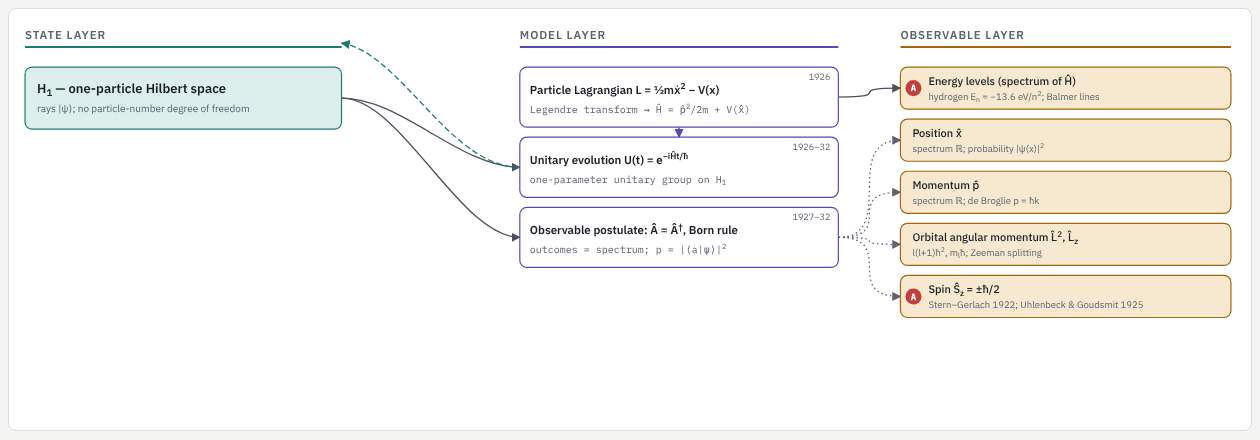
\includegraphics[width=\linewidth]{step01.png}\caption{Step 1. One state node, three model nodes, five observables (the Hermitian operators). The dashed teal arrow is the back-edge of unitary evolution.}\label{fig:s1}\end{figure}

\subsection*{Step 2 (1926--1939): Poincaré symmetry and Wigner's classification}
Requiring $U$ to represent the Poincaré group makes $\mathcal H_1$ decompose into irreducible subspaces. Wigner~\cite{Wigner1939} classified them by the little group of a standard momentum: SO(3) for $m>0$ (spin $s$), ISO(2) for $m=0$ (helicity $h$, or the continuous-spin representations), plus the tachyonic and trivial classes. The relativistic wave equations~\cite{Klein1926,Gordon1926,Dirac1928} are the equations satisfied by the carrier fields of these representations~\cite{BargmannandWigner1948,Weinberg1995}. Graph operation: \textsc{partition} of the state node by the back-edge of $U(\Lambda,a)$; mass and spin, the Casimir invariants, become observables with badge P (Figure~\ref{fig:s2}). Nine representation classes are drawn; the ones with a known instance in 1939 are the massive spin-$\tfrac12$ class (e, p, n, $\mu$), the massless helicity-1 class ($\gamma$) and, as a hypothesis, the massless helicity-$\tfrac12$ class ($\nu$). \emph{Order note.} The field quantization of Step~4 (1927--32) predates Wigner's paper. The step order follows logical dependence (the field is built on the representation) and every node carries its own date.

\begin{figure}[htbp]\centering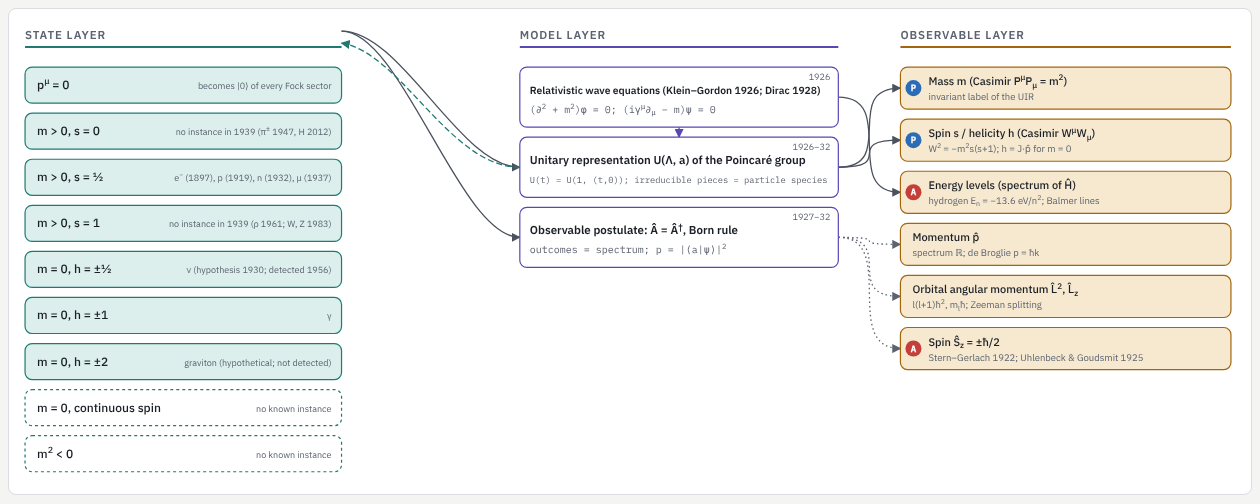
\includegraphics[width=\linewidth]{step02.png}\caption{Step 2. The state layer partitioned into Wigner's representation classes; classes without an instance are dashed. Mass and spin appear as observables.}\label{fig:s2}\end{figure}

\subsection*{Step 3 (1914--1934): an observable with no model edge}
Three observations share one feature: the final state contains a different number of particles than the initial one. Emission and absorption of light, quantified by Einstein's $A$ and $B$ coefficients~\cite{Einstein1917}; $\beta$ decay with a continuous electron spectrum~\cite{Chadwick1914,EllisandWooster1927}, where the electron is not a nuclear constituent; and $e^+e^-$ pairs created by $\gamma$ rays~\cite{Anderson1933,BlackettandOcchialini1933}. Since $U(\Lambda,a)$ acts within $\mathcal H_1$, and even within a single representation, no node of the model layer can send an edge to this observable. Graph operation: \textsc{add} an observable node with in-degree zero from the model layer (Figure~\ref{fig:s3}, red dashed ring). This is the first firing of the rule that drives the whole evolution (Rule~2 in Section~\ref{sec:laws}).

\begin{figure}[htbp]\centering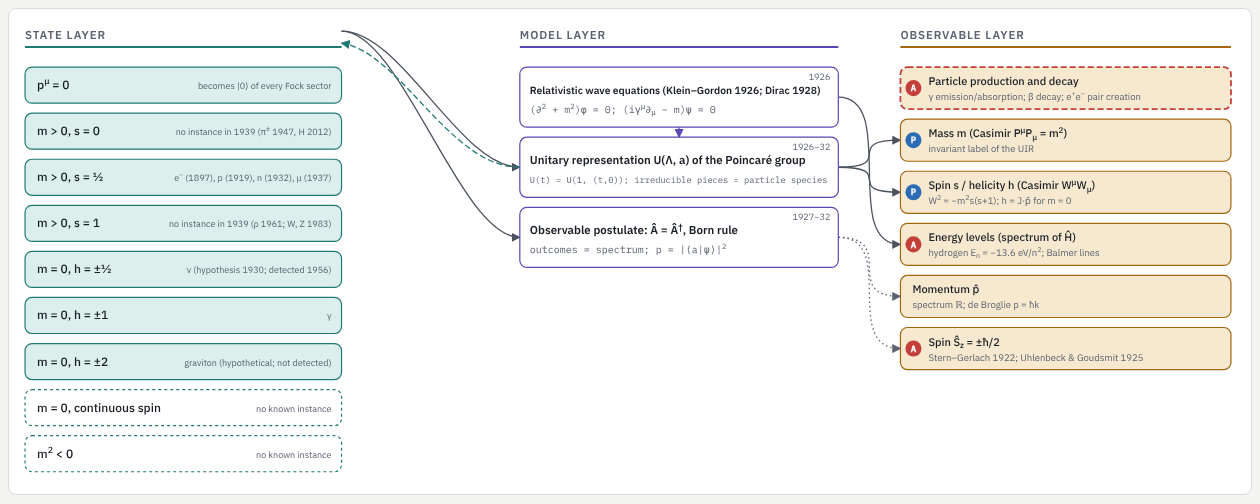
\includegraphics[width=\linewidth]{step03.png}\caption{Step 3. The observable ``particle production and decay'' has no incoming model edge.}\label{fig:s3}\end{figure}

\subsection*{Step 4 (1927--1940): quantum fields on Fock space}
The repair is a model node that adds or removes one quantum of a given representation: the quantum field $\phi(x)=\sum_p(a_p u_p+a_p^\dagger u_p^*)$. Dirac~\cite{Dirac1927} built the photon field this way to derive Einstein's $A$ coefficient; Jordan and Wigner~\cite{JordanandWigner1928} gave the fermionic construction, Heisenberg and Pauli~\cite{HeisenbergandPauli1929} the general Lagrangian field theory, Fock~\cite{Fock1932} the space $\bigoplus_N \mathrm{Sym}^N\mathcal H_1$ (bosons) or $\bigoplus_N\Lambda^N\mathcal H_1$ (fermions), and Fierz~\cite{Fierz1939} and Pauli~\cite{Pauli1940} the connection between spin and statistics. Graph operations: \textsc{add} the field node (the one-particle Lagrangian merges into it as the free-field Lagrangian $L_0$), and \textsc{extend} every realized representation into a sector with the ladder $|0\rangle,|1\rangle,|2\rangle,\dots,|N\rangle$ by the new back-edge (Figure~\ref{fig:s4}). The observable layer changes character: the observables of interest are now transition rates, $\Gamma=2\pi|\langle f|H_{\rm int}|i\rangle|^2\rho(E)$ and $\sigma\propto|\langle f|S|i\rangle|^2$~\cite{Wheeler1937,Heisenberg1943,Dyson1949}. They remain unexplained at this step: with $L_{\rm int}=0$ the S-matrix is~1. The free field explains that particle number can change, not which processes occur.

\begin{figure}[htbp]\centering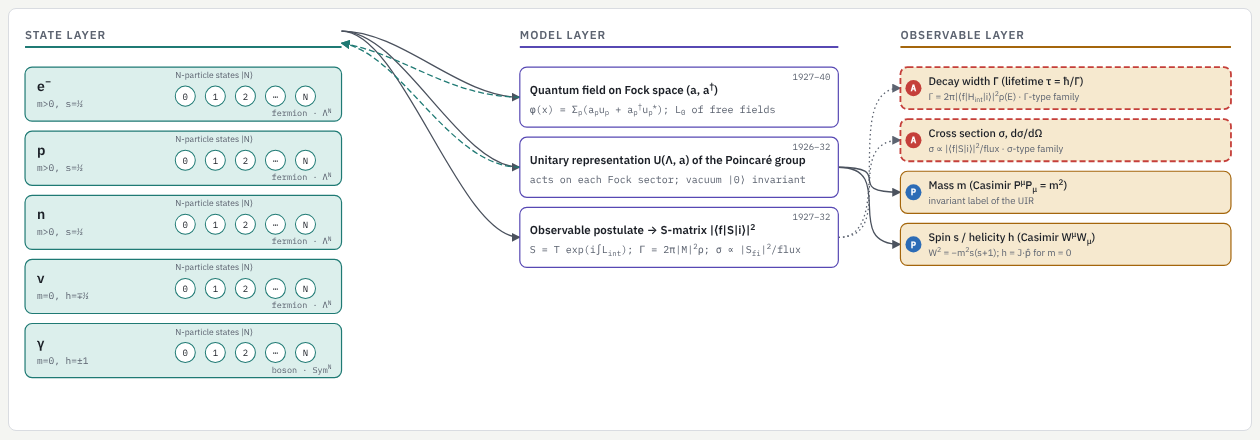
\includegraphics[width=\linewidth]{step04.png}\caption{Step 4. Each realized representation becomes a Fock sector with an occupation ladder; the field node sends the back-edge that builds the ladders. $\Gamma$ and $\sigma$ are still unexplained.}\label{fig:s4}\end{figure}

\subsection*{Step 5 (1927--1949): the QED vertex}
Minimal coupling $p\to p-eA$ applied to the quantized fields gives the single term $-e\bar\psi\gamma^\mu\psi A_\mu$~\cite{Dirac1927,HeisenbergandPauli1929}. One vertex changes $N_\gamma$ by $\pm1$ and $N_e$ by $0$ or $\pm2$; the route is drawn from the minimal configuration $e(1)\wedge\gamma(1)$. At order $\alpha$ the node reproduces the Klein--Nishina cross section~\cite{KleinandNishina1929} and the Bethe--Heitler pair-production cross section~\cite{BetheandHeitler1934}; at order $\alpha^2$ the renormalized theory~\cite{Tomonaga1946,Schwinger1948,Feynman1949,Dyson1949} gives $a_e=\alpha/2\pi=0.00116$ against the measured $0.00119(5)$~\cite{KuschandFoley1948} and a Lamb shift of about 1040~MHz~\cite{Bethe1947} against about 1000~MHz measured~\cite{LambandRetherford1947}. The coupling is not predicted: the edge to $\alpha$ is a calibration (F). Pair production carries badge P (Dirac's hole theory~\cite{Dirac1931} preceded Anderson), the other three carry A. $\beta$ decay stays unexplained (Figure~\ref{fig:s5}).

\begin{figure}[htbp]\centering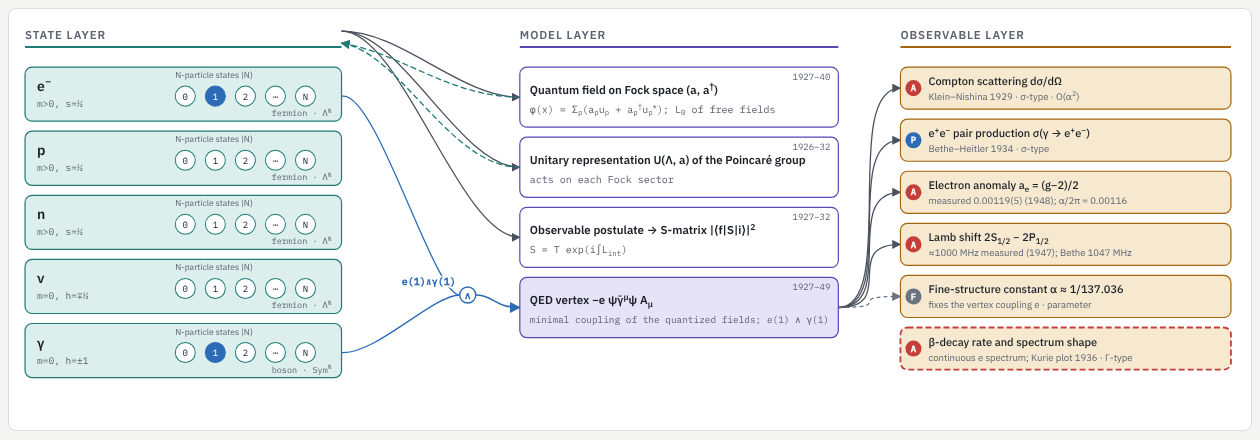
\includegraphics[width=\linewidth]{step05.png}\caption{Step 5. The first AND route, $e(1)\wedge\gamma(1)$, enters the QED vertex, which reaches four observables and calibrates $\alpha$.}\label{fig:s5}\end{figure}

\subsection*{Step 6 (1934): Fermi's contact term}
Fermi~\cite{Fermi1934a,Fermi1934b} copied the structure of the QED vertex: a nucleon current $\bar p\gamma^\mu n$ in place of the electron current and the pair $(e,\bar\nu)$ created at a point in place of the photon. The spectrum shape follows from phase space and the matrix element (Kurie plot~\cite{Kurieetal1936}); Gamow and Teller~\cite{GamowandTeller1936} added axial-vector and tensor structure. The route $n(1)\wedge p(1)\wedge e(1)\wedge\bar\nu(1)$ is the first with four legs (Figure~\ref{fig:s6}). The coupling $G_F\approx1.166\times10^{-5}\,\mathrm{GeV}^{-2}$ has dimension mass$^{-2}$: the amplitude grows like $G_F s$ and partial-wave unitarity fails at $\sqrt s$ of a few hundred GeV (a textbook argument), so the node is \emph{effective} and is drawn dashed. The neutron lifetime carries P~\cite{ChadwickandGoldhaber1935,Robson1951}; the neutrino itself was detected in 1956~\cite{Cowanetal1956}.

\begin{figure}[htbp]\centering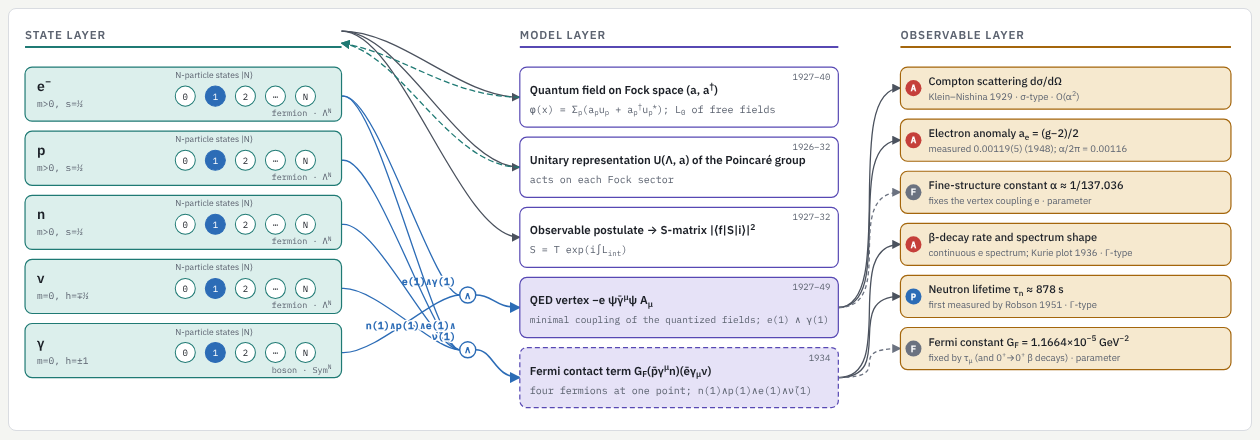
\includegraphics[width=\linewidth]{step06.png}\caption{Step 6. Fermi's effective node (dashed) with its four-leg route; $G_F$ is a calibration.}\label{fig:s6}\end{figure}

\subsection*{Step 7 (1937--1962): the muon and universality}
The muon~\cite{NeddermeyerandAnderson1937} was first taken for Yukawa's meson; Conversi, Pancini and Piccioni~\cite{Conversietal1947} showed that it does not interact strongly. Its decay is a second four-fermion node. The decisive fact is that one constant fits $\beta$ decay, $\mu$ decay and $\mu$ capture~\cite{Puppi1948,Klein1948,TiomnoandWheeler1949,LeeRosenbluthandYang1949}; $\tau_\mu^{-1}=G_F^2m_\mu^5/192\pi^3$ makes $\tau_\mu$ the most precise source of $G_F$, so the calibration edge moves to the muon node. Michel~\cite{Michel1950} parametrized the electron spectrum. Danby et al.~\cite{Danbyetal1962} showed that neutrinos from $\pi\to\mu\nu$ produce muons and not electrons: graph operation \textsc{split} of the $\nu$ sector into $\nu_e$ and $\nu_\mu$ (Figure~\ref{fig:s7}). Two model nodes sharing one coupling is the signal that they are instances of one node (Rule~6).

\begin{figure}[htbp]\centering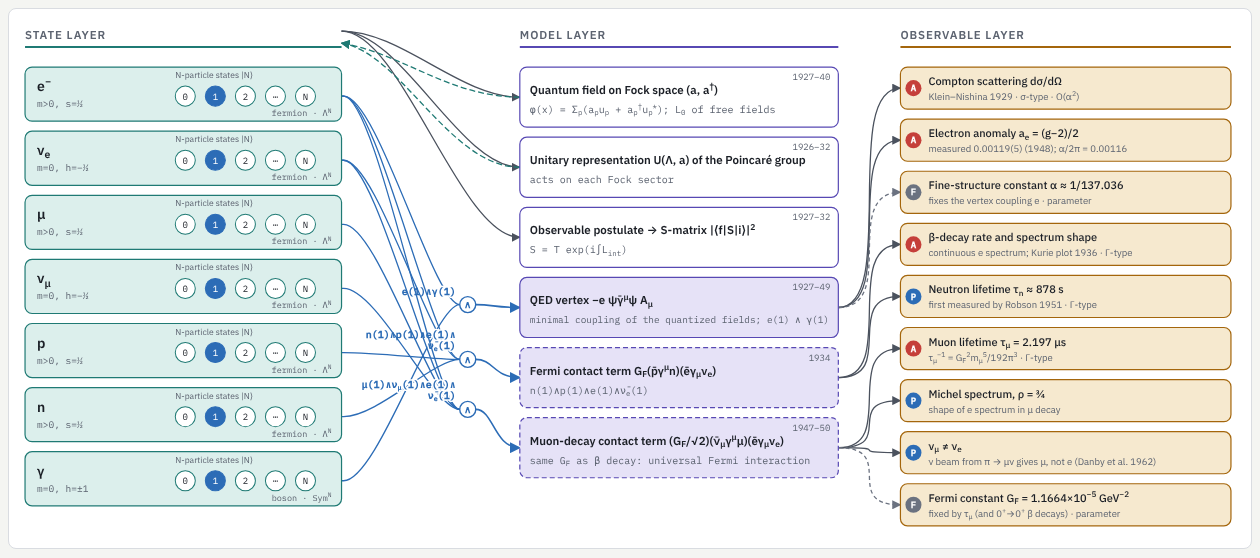
\includegraphics[width=\linewidth]{step07.png}\caption{Step 7. A $\mu$ sector and two neutrino sectors; two effective nodes share $G_F$.}\label{fig:s7}\end{figure}

\subsection*{Step 8 (1956--1958): parity violation and V$-$A}
The $\tau$--$\theta$ puzzle led Lee and Yang~\cite{LeeandYang1956} to propose tests of parity in weak processes; Wu et al.~\cite{Wuetal1957} and Garwin, Lederman and Weinrich~\cite{Garwinetal1957} found the asymmetries. No parity-conserving node can produce a pseudoscalar correlation, so the new observables are unexplained until Feynman and Gell-Mann~\cite{FeynmanandGellMann1958} and Sudarshan and Marshak~\cite{SudarshanandMarshak1958} replace the two contact nodes by one current--current term with vector-minus-axial currents, which fixes $\rho=\tfrac34$ and the neutrino helicity $-1$~\cite{Goldhaberetal1958}; the hadronic current later acquires $\cos\theta_C$~\cite{Cabibbo1963}. Graph operation: \textsc{merge} of the two effective nodes into one, entered by three routes ($\beta$ decay, $\mu$ decay, $\mu$ capture) (Figure~\ref{fig:s8}).

\begin{figure}[htbp]\centering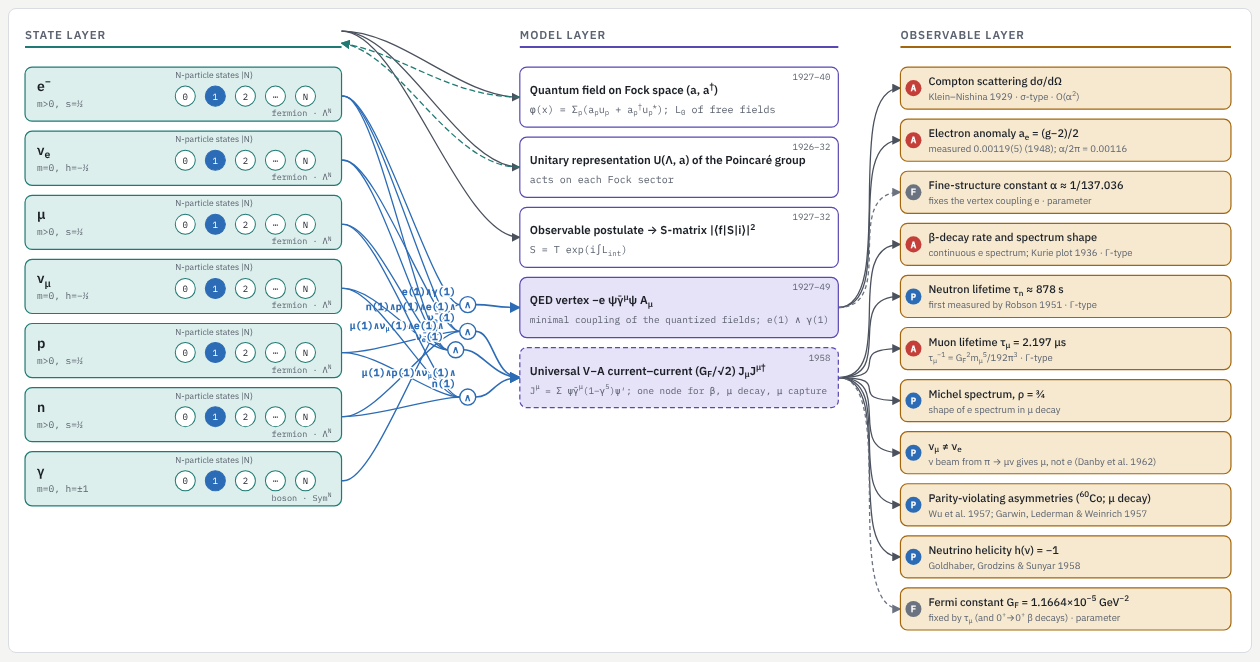
\includegraphics[width=\linewidth]{step08.png}\caption{Step 8. One V$-$A node replaces two contact nodes; three AND routes enter it.}\label{fig:s8}\end{figure}

\subsection*{Step 9 (1954--1983): W, Z and SU(2)$_L\times$U(1)$_Y$}
Replacing the contact term by the exchange of a massive vector boson~\cite{Schwinger1957,Bludman1958} and demanding a renormalizable gauge structure~\cite{YangandMills1954,Glashow1961,Weinberg1967,Salam1968,tHooft1971,tHooftandVeltman1972} turns the effective node into the low-energy limit of a fundamental one: $G_F/\sqrt2=g^2/8M_W^2$, the four-fermion node being recovered for $q^2\ll M_W^2$ (the effective-field-theory reading of~\cite{Weinberg1979}). The same symmetry forces a neutral current, observed by Gargamelle~\cite{Hasertetal1973} ten years after the prediction, and W and Z production at the SPS~\cite{Arnisonetal1983,Banneretal1983,Arnisonetal1983b}. The nucleon current is rewritten at quark level~\cite{GellMann1964,Bloometal1969}; the QCD sector that binds $u,d$ into $n,p$ is outside this graph, so graph operation \textsc{replace} exchanges the $(n,p)$ sectors for $(u,d)$. The invisible Z width fixes $N_\nu=2.984\pm0.008$~\cite{LEPEWWG2006}, a model-layer prediction about the number of state-layer sectors; the gauge self-couplings were tested at LEP2~\cite{LEP2EWWG2013}. Graph operations: \textsc{absorb} (V$-$A into the charged current), \textsc{add} (neutral current, self-couplings, W and Z sectors), \textsc{replace}. From here the observables carry badge P: they were predicted before they were seen (Figure~\ref{fig:s9}).

\begin{figure}[htbp]\centering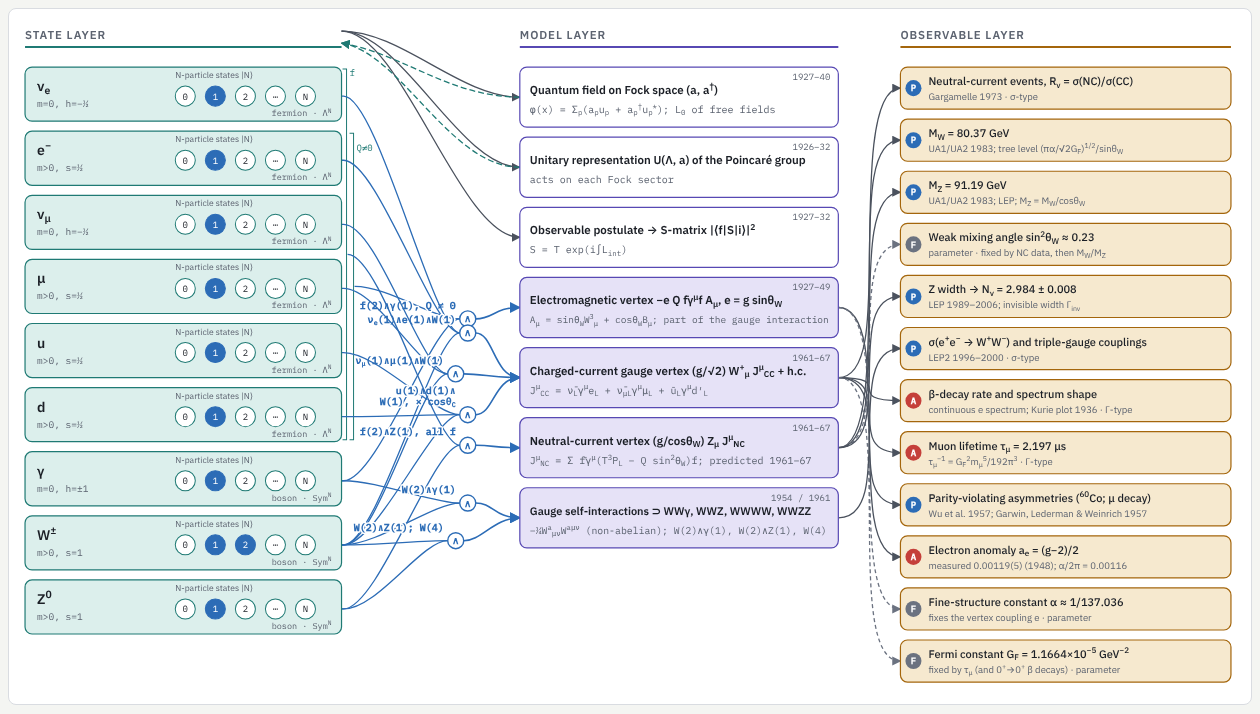
\includegraphics[width=\linewidth]{step09.png}\caption{Step 9. Fundamental vertices with dimensionless couplings; W and Z sectors; the $\beta$-decay route enters through $u(1)\wedge d(1)\wedge W(1)$. Observables are now predicted before observed.}\label{fig:s9}\end{figure}

\subsection*{Step 10 (1964--2012): the Higgs sector}
Explicit mass terms for W, Z and the chiral fermions are forbidden by the gauge symmetry. The Brout--Englert--Higgs mechanism~\cite{EnglertandBrout1964,Higgs1964,GuralnikHagenandKibble1964} adds a scalar doublet whose vacuum value $v=(\sqrt2G_F)^{-1/2}=246$~GeV gives $M_W=gv/2$, $M_Z=M_W/\cos\theta_W$ and, through Yukawa couplings, $m_f=y_fv/\sqrt2$~\cite{Weinberg1967}. The W and Z mass edges of Step~9 are now derived from the Higgs--gauge node. A scalar with $m_H^2=2\lambda v^2$ is predicted; ATLAS and CMS~\cite{ATLAS2012,CMS2012} observed it at 125~GeV and the measured rates match the Standard-Model pattern~\cite{PDG2024}. The fermion masses and $m_H$ remain inputs (calibrations); the trilinear coupling has not been measured, only bounded (Figure~\ref{fig:s10}).

\begin{figure}[htbp]\centering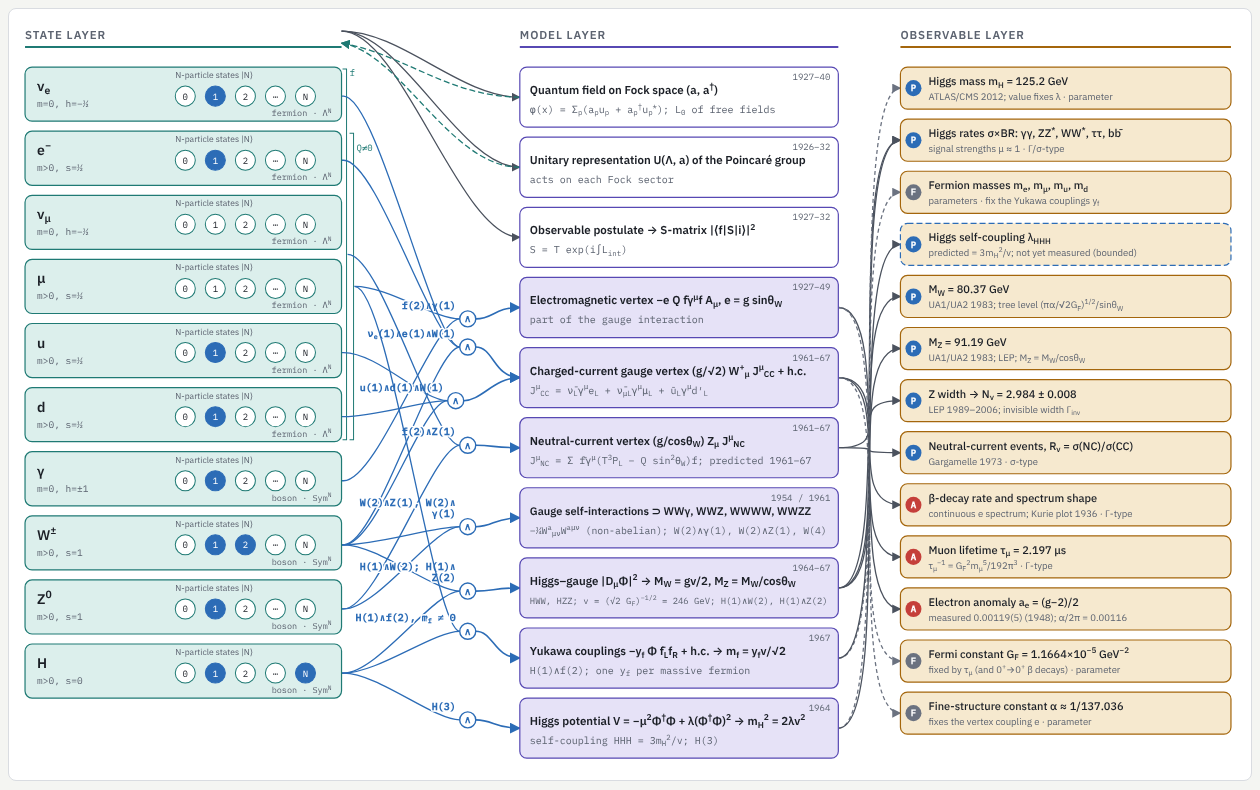
\includegraphics[width=\linewidth]{step10.png}\caption{Step 10. The H sector and the three Higgs-sector nodes; calibration edges for $m_f$ and $m_H$; the untested $\lambda_{HHH}$ has a blue dashed ring.}\label{fig:s10}\end{figure}

\subsection*{Step 11 (1998--): the frontier}
Super-Kamiokande~\cite{Fukudaetal1998}, SNO~\cite{Ahmadetal2002} and KamLAND~\cite{Eguchietal2003} established flavour oscillation, which requires non-degenerate neutrino masses. In the graph as built the $\nu$ sectors carry the massless representation (helicity $-\tfrac12$ only, no right-handed state), so no Yukawa node can reach them: the observable has in-degree zero from the model layer, the situation of Step~3 again. Candidate repairs are drawn dashed: the dimension-5 operator $(L\Phi)(L\Phi)/\Lambda$~\cite{Weinberg1979b}, which uses only existing sectors, or new $\nu_R$ sectors with Dirac Yukawa couplings and possibly Majorana masses~\cite{Minkowski1977,MohapatraandSenjanovi1980}. Current data do not decide between them (Figure~\ref{fig:s11}).

\begin{figure}[htbp]\centering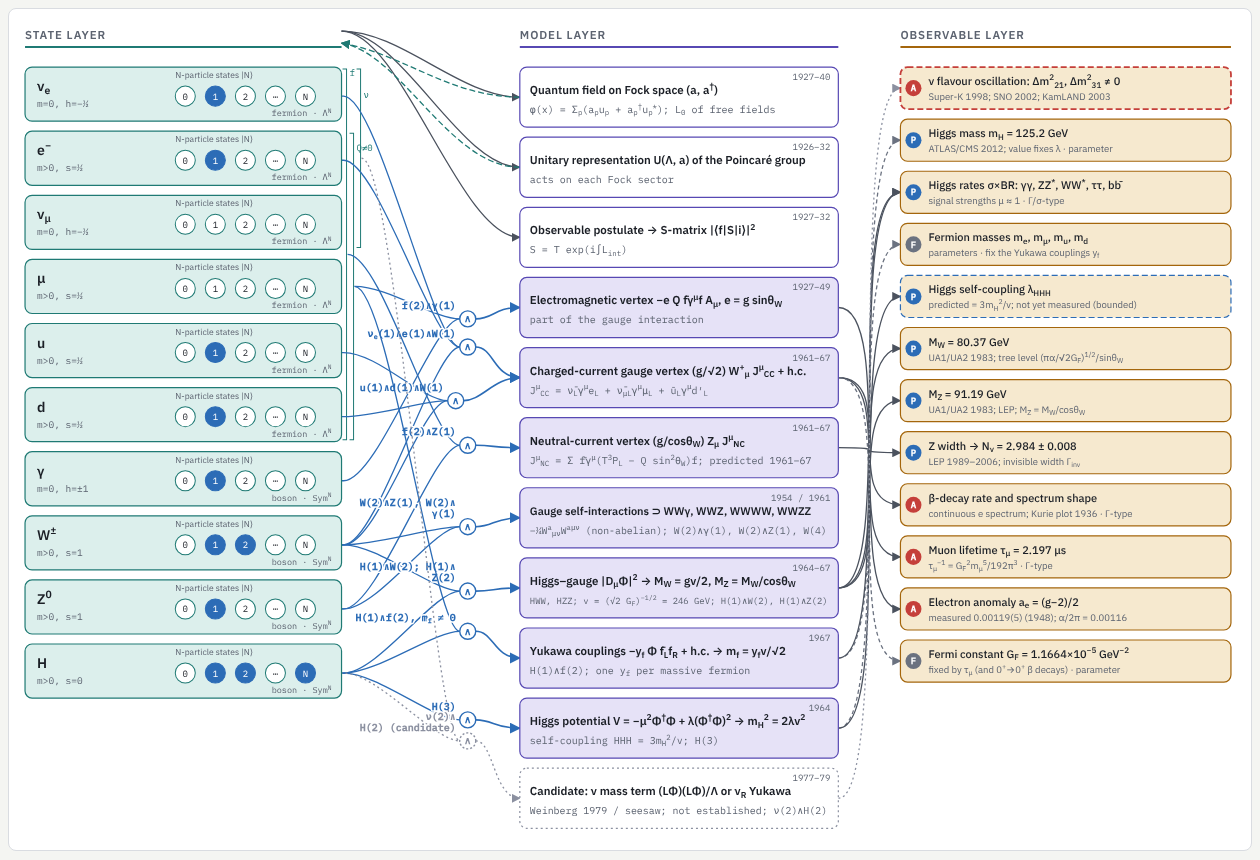
\includegraphics[width=\linewidth]{step11.png}\caption{Step 11. Neutrino oscillation is unexplained by the established nodes; the candidate node and its route are dashed.}\label{fig:s11}\end{figure}

\subsection*{Step 12: the Standard Model as clusters}
The final view groups the model layer by the five terms of
\begin{equation}
\mathcal L_{\rm SM}=-\tfrac14W^a_{\mu\nu}W^{a\mu\nu}-\tfrac14B_{\mu\nu}B^{\mu\nu}+\sum_f\bar f\,i\gamma^\mu D_\mu f+|D_\mu\Phi|^2-V(\Phi)-\big(y_f\bar f_L\Phi f_R+\text{h.c.}\big),
\end{equation}
plus one dashed cluster for the candidate neutrino-mass term. Each cluster is one term; its fundamental vertices are the members; and the effective nodes of Steps~6--8 sit inside the gauge--fermion cluster, greyed, with lineage edges Fermi$\to$V$-$A$\leftarrow\mu$-decay and V$-$A$\to$charged current (the matching condition $G_F/\sqrt2=g^2/8M_W^2$ is the edge). Routes from the sectors now enter the clusters: every fermion sector with $\gamma$, W or Z into the gauge--fermion term (five routes), W with $\gamma$ or Z into the gauge kinetic term, H with W, Z, the massive fermions or itself into the Higgs terms. Edges to observables leave the clusters (Figure~\ref{fig:s12}; Tables~\ref{tab:clusters} and~\ref{tab:routes}). Graph operation: \textsc{cluster}. The count at the end is \nFinalSectors{} sectors, \nFinalClusters{} clusters, \nFinalFund{} fundamental vertices, \nFinalAbsorbed{} absorbed effective nodes, \nFinalRoutes{} routes and \nFinalObs{} observables, of which \nFinalFit{} are calibrations, one is an untested prediction and one is unexplained.

\begin{figure}[htbp]\centering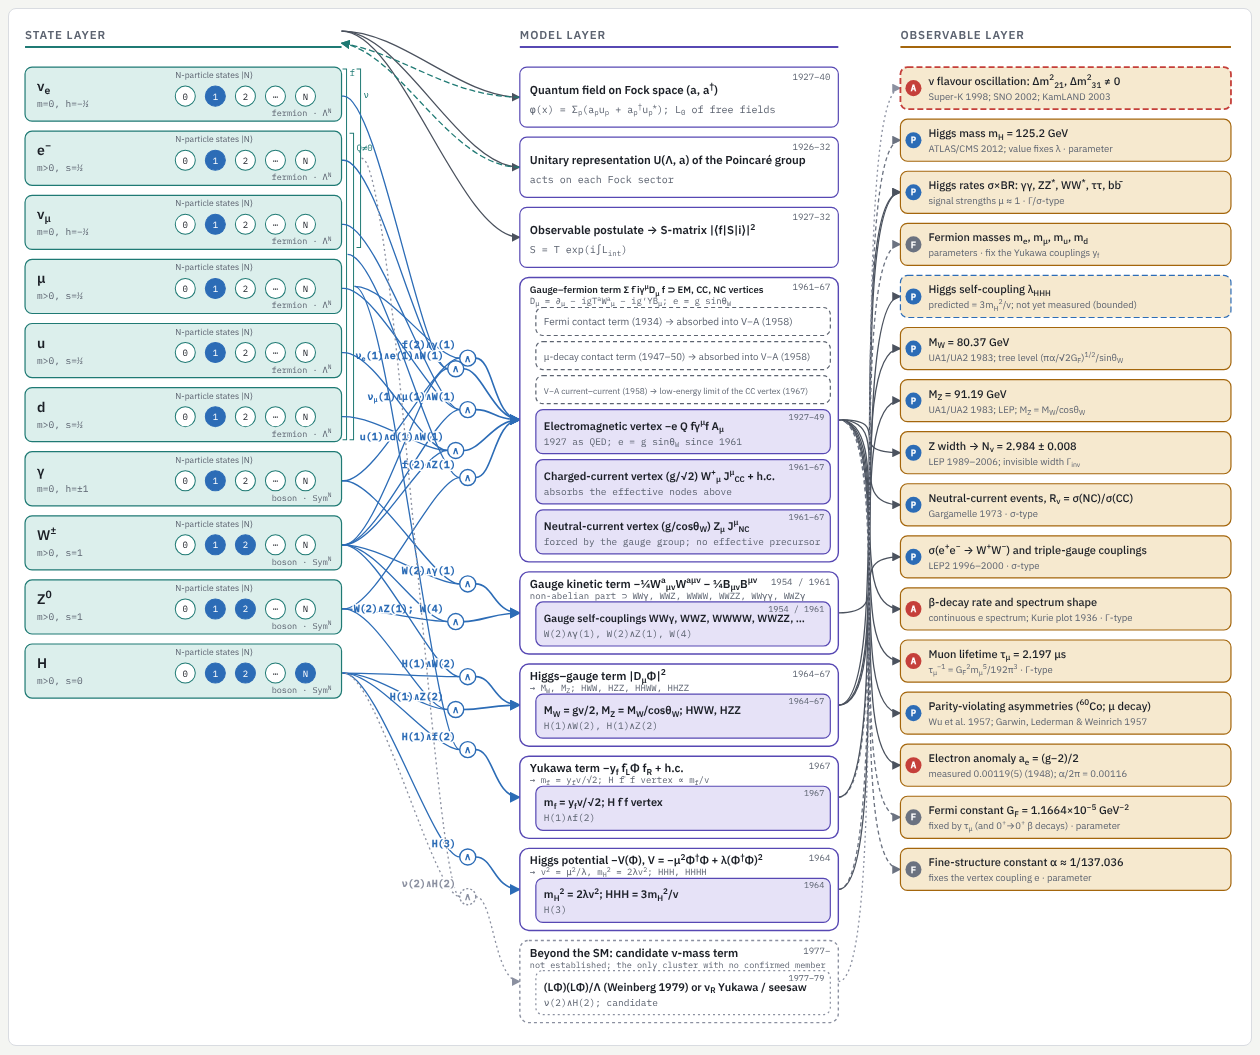
\includegraphics[width=\linewidth]{step12.png}\caption{Step 12. The model layer clustered by Lagrangian term. Greyed dashed chips inside the gauge--fermion cluster are the absorbed effective nodes; the dashed cluster at the bottom holds the candidate neutrino-mass term.}\label{fig:s12}\end{figure}

\subsection*{Step 13: synthesis, the method in action}
The synthesis view has two parts. The first, ``the method in action'' (Figures~\ref{fig:m4}, \ref{fig:m9} and~\ref{fig:m12}), shows the scientific method operating on the graph. On the left is the cycle observe $\to$ deficit $\to$ hypothesize $\to$ restructure $\to$ predict $\to$ calibrate $\to$ reduce, with the phases active in the chosen step filled and the regime of the step named (anomaly-first, prediction-first, symmetry-driven, model response, reduction). On the right the whole graph is drawn small and re-laid out at every step: a node added in the step carries a $+$ mark, a node rewritten a $\sim$ mark, new edges and routes are highlighted, and a removed node slides into the node that replaces or absorbs it. Under the pair, the step's operations on the graph are listed with their layer or edge kind (\textsc{add}, \textsc{partition}, \textsc{extend}, \textsc{split}, \textsc{replace}, \textsc{merge}, \textsc{absorb}, \textsc{cluster}, \textsc{route}, \textsc{predict}, \textsc{calibrate}, \textsc{flag}). A Play button runs the twelve steps as an animation. The phases and operations of each step are part of the data (\texttt{phases} and \texttt{ops} fields in the JSON), so the view is generated, not drawn by hand. The second part (Figure~\ref{fig:s13}) plots four counts against the step number and tabulates the changes per layer. The counts are the quantitative content of the rules in the next section.

\begin{figure}[htbp]\centering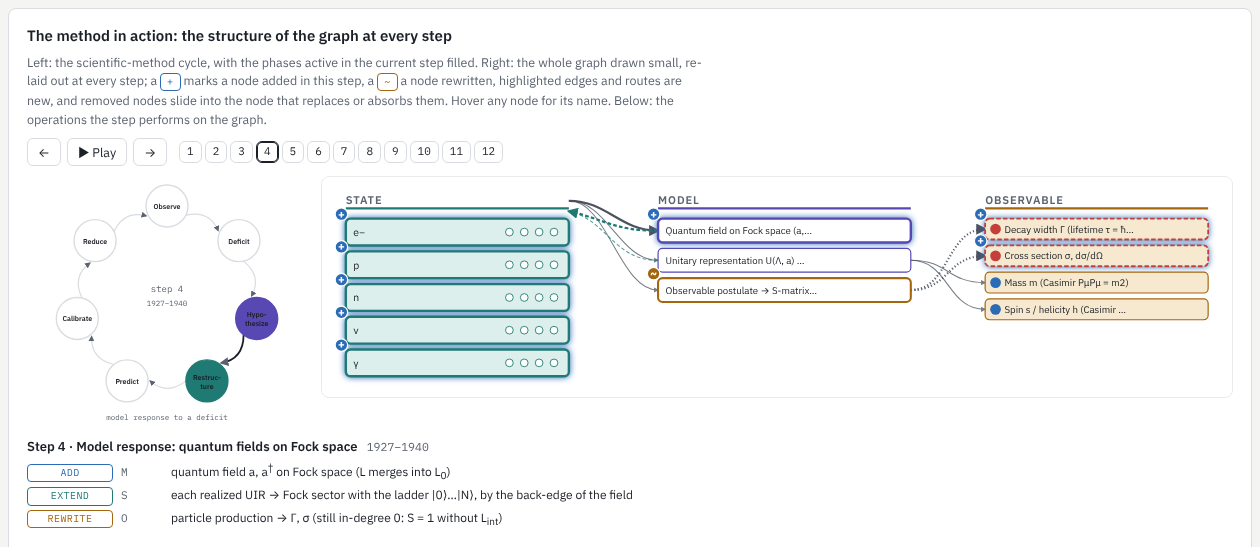
\includegraphics[width=\linewidth]{method_s4.png}\caption{The method in action at Step 4: the cycle shows hypothesize and restructure active (a model response to the deficit of Step 3); in the schematic every sector carries a $+$ (the ladders are new), the observable postulate is rewritten ($\sim$) and the two generic observables keep their red rings; the operation log reads \textsc{add}, \textsc{extend}, \textsc{rewrite}.}\label{fig:m4}\end{figure}
\begin{figure}[htbp]\centering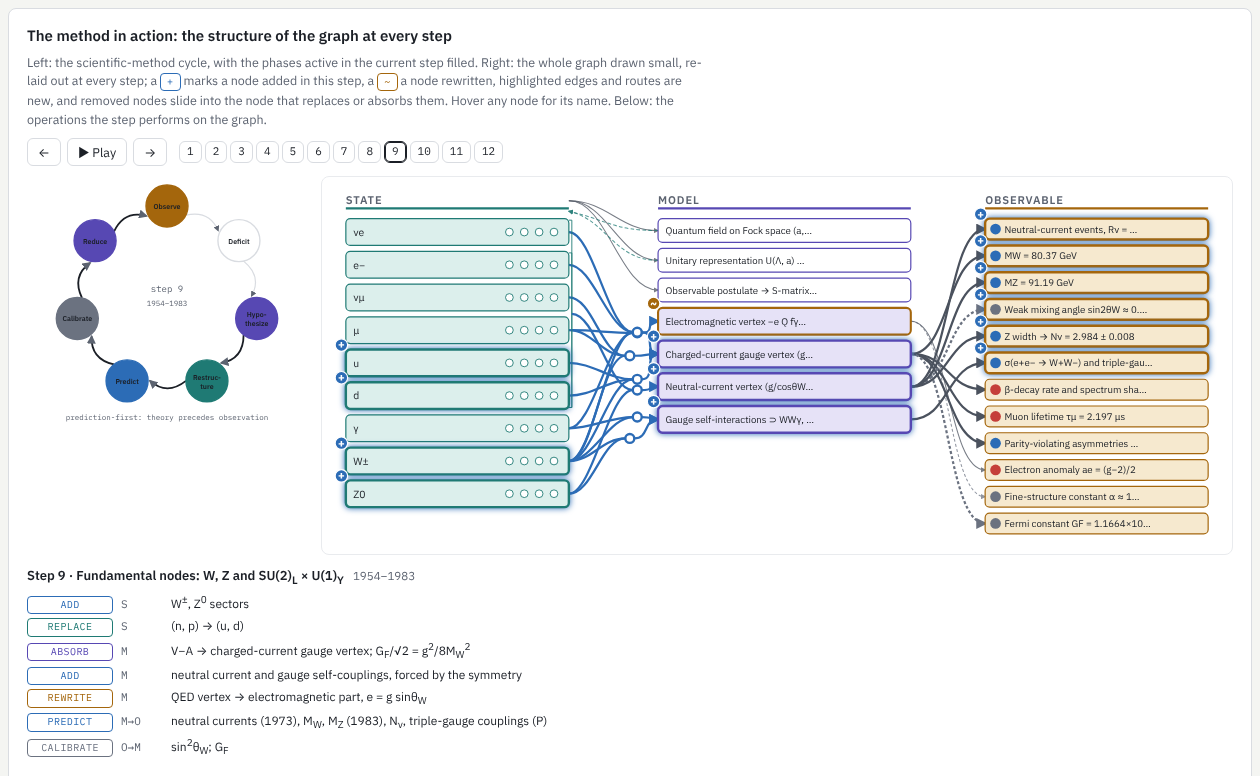
\includegraphics[width=\linewidth]{method_s9.png}\caption{The method in action at Step 9: six phases active (prediction-first regime); new sectors W, Z, u, d, new vertices, new routes and new predicted observables are highlighted; the log reads \textsc{add}, \textsc{replace}, \textsc{absorb}, \textsc{add}, \textsc{rewrite}, \textsc{predict}, \textsc{calibrate}.}\label{fig:m9}\end{figure}
\begin{figure}[htbp]\centering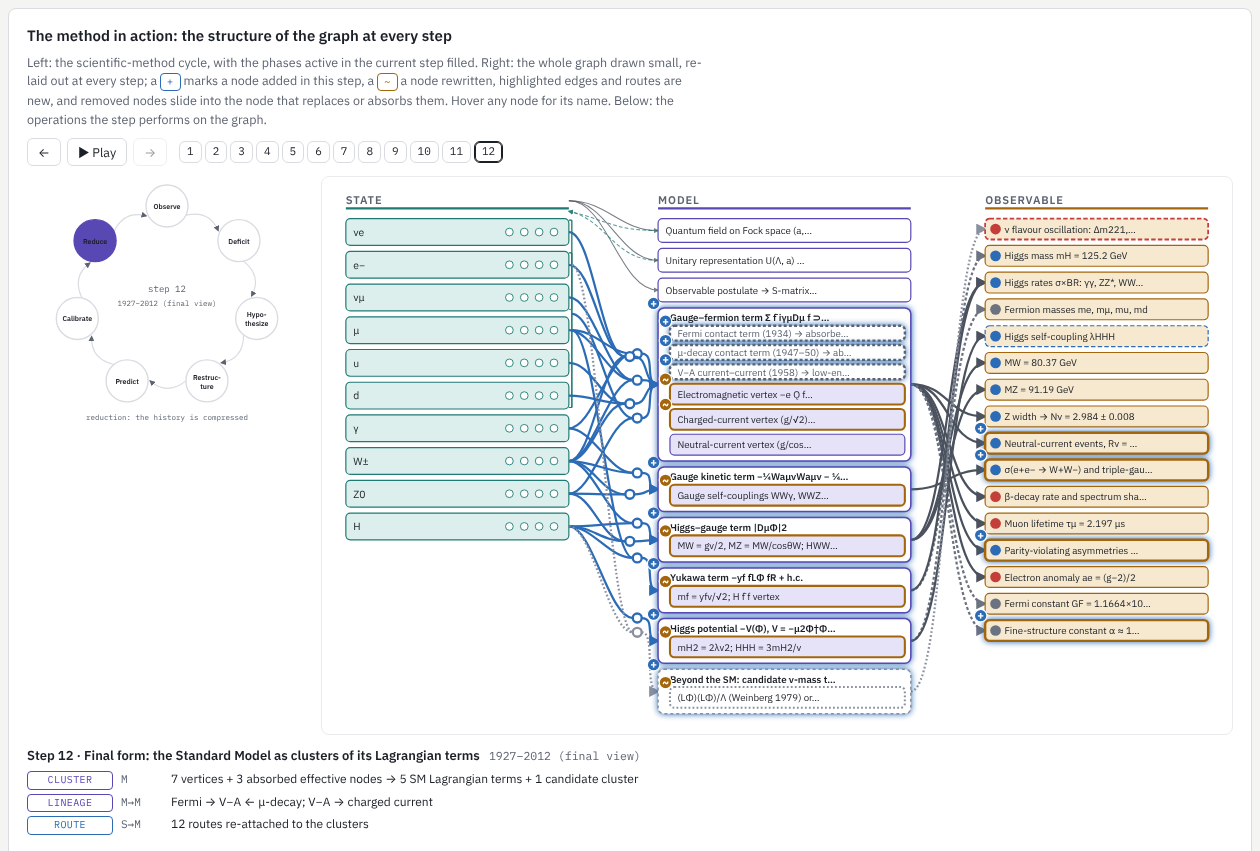
\includegraphics[width=\linewidth]{method_s12.png}\caption{The method in action at Step 12: only reduce is active; the schematic shows the clusters with the absorbed nodes inside and all routes re-attached.}\label{fig:m12}\end{figure}
\begin{figure}[htbp]\centering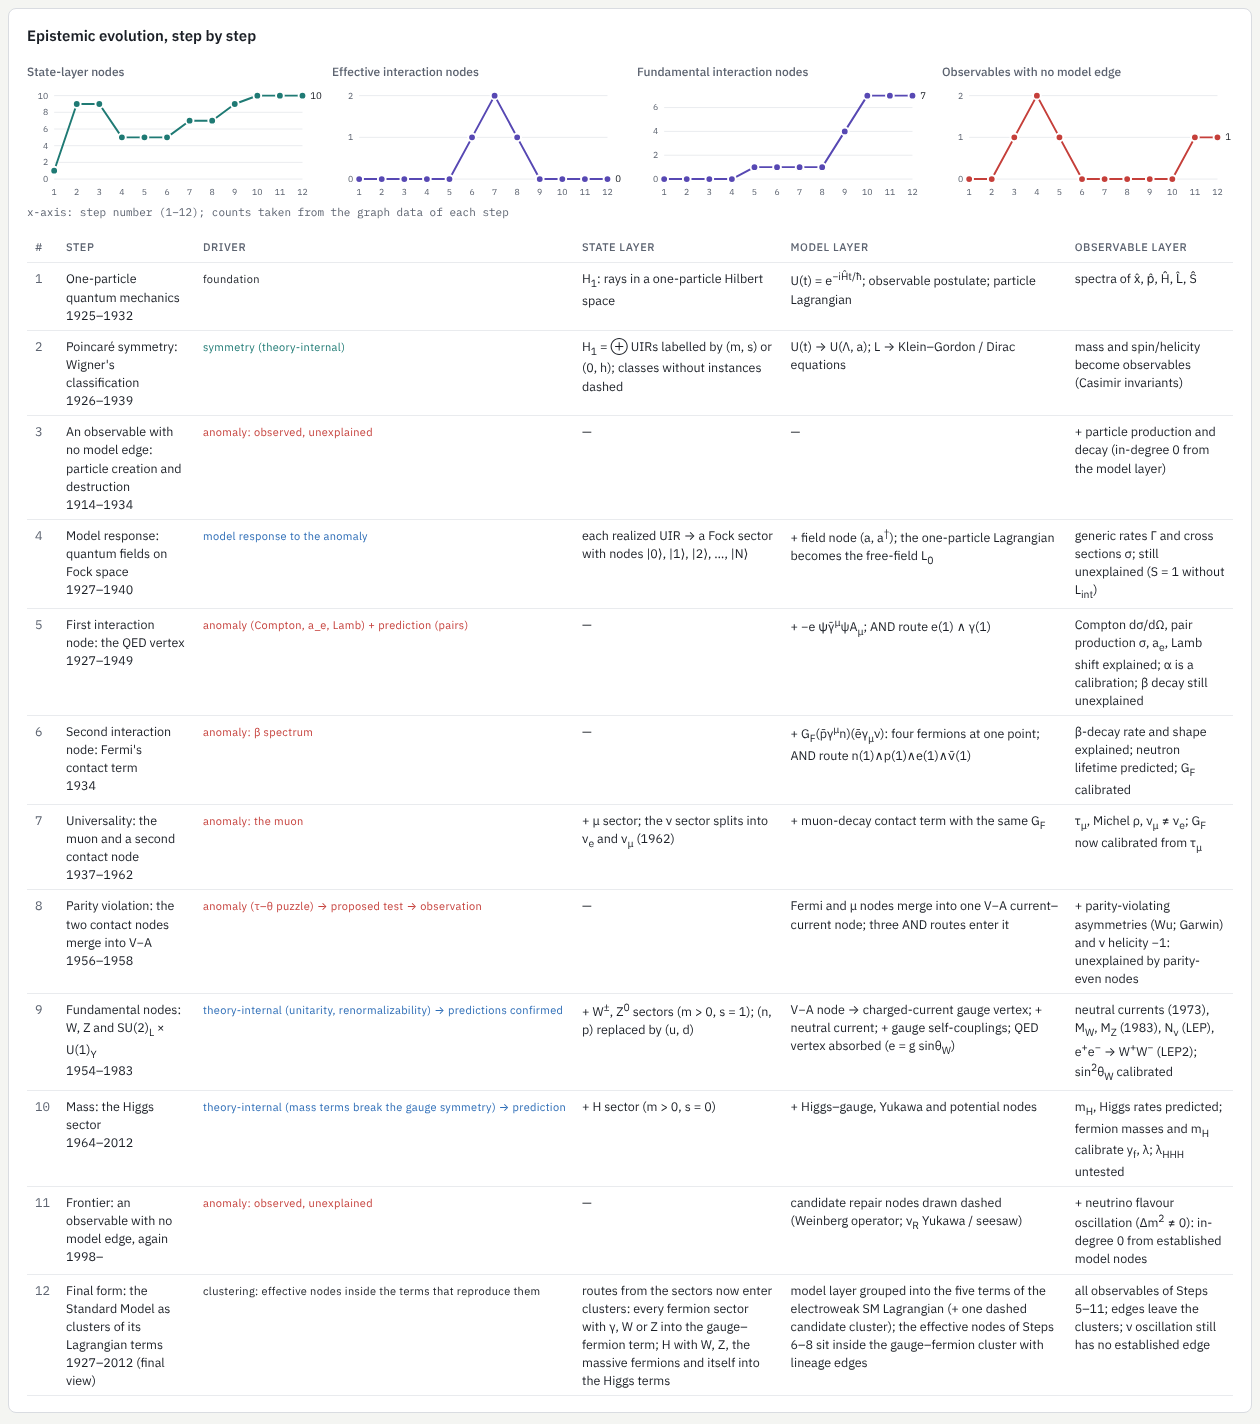
\includegraphics[width=\linewidth]{step13.png}\caption{Step 13, second part. Counts per step: state-layer nodes, effective interaction nodes outside clusters, fundamental interaction nodes, observables with no model edge.}\label{fig:s13}\end{figure}

\section{Rules of evolution}\label{sec:laws}

The sequence of Section~\ref{sec:history} is not arbitrary. Reading the twelve steps as graph operations, the same few rules fire again and again. We state each rule in graph terms, give the step(s) in which it fires, and say what it would predict for an instance not yet built. Notation: $N^-_M(o)$ is the set of model nodes with an edge into the observable $o$ (framework assignments and candidate edges excluded); $\dim[g]$ is the mass dimension of the coupling of a model node; a \emph{route} $(L,m)$ has legs $L\subset V_S\times\mathbb N$ and head $m\in V_M$. The rules are regularities of this instance and are written so that they can fail on the next.

\paragraph{Rule 1 (symmetry partition).} \emph{If a framework node represents a symmetry group $G$ unitarily on a state node, the state node is replaced by the irreducible components of the representation, and the labels of the components (the Casimir invariants) become observables.} Fires at Step~2: $U(\Lambda,a)$ partitions $\mathcal H_1$ into Wigner's classes; $P^2=m^2$ and $W^2=-m^2s(s+1)$ become observables with badge P. The irreducible components are the \emph{building blocks} of the state layer: no model node maps one of them into a proper subspace of itself. Prediction for other instances: wherever a symmetry is imposed on the state layer (isospin SU(2), flavour SU(3), colour SU(3)), the state nodes split into multiplets and a new label becomes an observable.

\paragraph{Rule 2 (in-degree-zero drive).} \emph{A model node is added only when there exists an observable node $o$ with $N^-_M(o)=\emptyset$, or when the existing model layer is inconsistent on theory-internal grounds. In the first case the new node must send an edge to $o$; in the second it must reproduce every edge of the node it replaces.} Fires at Steps~3$\to$4 (particle production $\to$ field node), 5 (Compton, $a_e$, Lamb $\to$ QED vertex), 6 ($\beta$ spectrum $\to$ Fermi), 7 (muon lifetime $\to$ second contact node), 8 (parity asymmetries $\to$ V$-$A), 11 (oscillation $\to$ candidate node); the theory-internal case fires at Steps~9 (non-renormalizability and unitarity $\to$ gauge vertices) and 10 (forbidden mass terms $\to$ Higgs sector). In the graph, the red dashed ring is a to-do item for the model layer. The rule also says what \emph{never} happens: no model node is added with no observable to reach and no inconsistency to cure.

\paragraph{Rule 3 (Fock extension).} \emph{If the repairing model node must connect states of different particle number, the state layer is extended by the model node's back-edge: every irreducible block $\mathcal H_s$ becomes the ladder $\bigoplus_N \mathrm{Sym}^N\mathcal H_s$ or $\bigoplus_N\Lambda^N\mathcal H_s$, and no new irreducible block is introduced.} Fires at Step~4. Two features are worth stating. The extension is \emph{minimal}: it composes existing building blocks (tensor powers) rather than inventing new ones, which is why the sectors of Step~4 are exactly the representations of Step~2 with a ladder attached. And the trigger is \emph{relativistic}: the three observations of Step~3 involve energies at or above a creation threshold ($E\ge mc^2$ for pairs, the mass difference of the nucleus in $\beta$ decay, photon energy in emission). Non-relativistic observables never force this extension, which is why one-particle quantum mechanics was complete for atomic spectroscopy. Prediction: any instance whose observables involve number-changing transitions (phonons in solids, photons in cavity QED) must acquire ladders by the same operation.

\paragraph{Rule 4 (route composition).} \emph{Every interaction node $m$ is entered by routes whose legs are the (sector, occupation-number) pairs of the fields in the Lagrangian term of $m$; the occupation numbers are the minimal changes the term can effect; and the number of distinct routes into $m$ equals the number of sector combinations the term couples.} Fires from Step~5 on. The QED vertex has one route ($e(1)\wedge\gamma(1)$); Fermi's node one four-leg route; the V$-$A node three routes (the three processes it unifies); the charged-current vertex three routes (two lepton doublets and one quark doublet); the neutral-current vertex one route with a group leg (all fermions). The rule turns a Lagrangian into a set of hyperedges mechanically, and it is the rule an AI system can apply without judgement: the legs are read off the field content of the term.

\paragraph{Rule 5 (effective status).} \emph{A model node whose coupling has $\dim[g]<0$ is effective: it has a validity scale $\Lambda\sim|g|^{-1/|\dim g|}$, its observable edges are valid only for $q^2\ll\Lambda^2$, and it cannot be the final form of the model layer.} Fires at Steps~6--8 ($G_F$, $\dim=-2$, $\Lambda$ of a few hundred GeV). The rule is the graph form of the statement that non-renormalizable terms are low-energy limits; it marks the dashed nodes as temporary the moment they are added.

\paragraph{Rule 6 (universality merge).} \emph{Two model nodes that share a calibration edge (the same observable fixes the same parameter of both) are merged into one node whose routes are the union of theirs.} Fires at Step~8, prepared at Step~7: the Fermi and muon-decay nodes share $G_F$, and the V$-$A node that replaces them is entered by the union of their routes plus the $\mu$-capture route. In the graph, parameter identity is node identity. Prediction: wherever two effective nodes are calibrated by one measured constant, a merge is due; the merged node has fewer parameters and more routes.

\paragraph{Rule 7 (absorption).} \emph{An effective node $m_{\rm eff}$ is absorbed by a fundamental node $m_{\rm fund}$ with $\dim[g]=0$ together with a new mediator sector $s$ such that (i) $m_{\rm eff}$ is the $q^2\ll M_s^2$ limit of $m_{\rm fund}$ (the matching condition is a lineage edge), (ii) the routes of $m_{\rm eff}$ become routes of $m_{\rm fund}$ with an extra leg $s(1)$, and (iii) the symmetry that makes $g$ dimensionless forces further model nodes whose observables carry badge~P.} Fires at Step~9: V$-$A $\to$ charged current, $G_F/\sqrt2=g^2/8M_W^2$, the four-leg routes become three-leg routes with $W(1)$, and the gauge group forces the neutral current and the self-couplings, with the neutral-current events, $M_W$, $M_Z$, $N_\nu$ and the triple-gauge couplings all predicted before observed. Absorption is the inverse of proliferation: the effective count in Figure~\ref{fig:s13} goes $0,1,2,1,0$ while the fundamental count rises monotonically.

\paragraph{Rule 8 (sector refinement).} \emph{The state layer changes only from outside itself: by Rule~1 (symmetry), by Rule~3 (a model node's back-edge), or by an observable that distinguishes sectors, in which case a sector is split, or replaced if the observable shows compositeness.} Fires at Steps~7 (the $\nu$ sector splits into $\nu_e$, $\nu_\mu$ after Danby et al.), 9 ($n,p$ replaced by $u,d$ after deep inelastic scattering) and 11 (the $\nu$ sectors must change because the massless representation cannot carry $\Delta m^2\neq0$). No sector was ever added by a model node alone; the W, Z and H sectors were added by absorption (Rule~7) and by the theory-internal case of Rule~2, and each was then confirmed by an observable with badge~P.

\paragraph{Rule 9 (calibration).} \emph{A model node with $p$ free parameters needs $p$ calibration edges (badge F); its predictive content is the number of its observable edges minus $p$.} In the final graph the calibration edges are $\alpha$ and $G_F$ (gauge--fermion cluster), $\sin^2\theta_W$ (fixed at Step~9), the fermion masses (Yukawa cluster) and $m_H$ (potential). Every other model$\to$observable edge is a prediction. The rule locates the predictive power of a theory in the graph: it is the excess of solid edges over dashed ones leaving a cluster.

\paragraph{Rule 10 (clustering).} \emph{When the model layer contains no effective node outside a fundamental one, the fundamental nodes are grouped by Lagrangian term; an absorbed effective node sits inside the cluster whose member reproduces it; routes and observable edges are attached to the cluster; and the number of clusters equals the number of terms of the Lagrangian.} Fires at Step~12. The clustered graph is the final form of a theory in GEN: it is what remains when the history is forgotten, and the lineage edges inside a cluster are the only trace of the history that the final form keeps.

\paragraph{The cycle.} Rules 2--7 compose into a loop that the graph runs twice. An observable with in-degree zero appears (Rule~2); a model node repairs it and, if needed, extends the state layer (Rule~3); the node's routes are read off its term (Rule~4); if the coupling is dimensionful the node is temporary (Rule~5); nodes that share a coupling merge (Rule~6); the merged node is absorbed by a fundamental one with a new sector, and the symmetry that makes the coupling dimensionless predicts further observables (Rule~7); the fundamental nodes cluster (Rule~10). The first run of the loop is anomaly-first (Steps~3--8, badges~A); its second half is prediction-first (Steps~9--10, badges~P); Step~11 opens a third run with a new in-degree-zero observable. Table~\ref{tab:rules} records where each rule fires, and the method view of Step~13 (Figures~\ref{fig:m4}--\ref{fig:m12}) shows the loop running: at each step the active phases of the cycle are filled and the operations applied to the graph are listed.

\begin{table}[htbp]\centering\small
\caption{Where each rule fires.}\label{tab:rules}
\begin{tabular}{@{}lll@{}}\toprule
Rule & Operation & Steps \\\midrule
1 symmetry partition & \textsc{partition} & 2 \\
2 in-degree-zero drive & \textsc{add} (model) & 3$\to$4, 5, 6, 7, 8, 11; theory-internal: 9, 10 \\
3 Fock extension & \textsc{extend} & 4 \\
4 route composition & routes & 5, 6, 7, 8, 9, 10, 11, 12 \\
5 effective status & marking & 6, 7, 8 \\
6 universality merge & \textsc{merge} & 8 (prepared in 7) \\
7 absorption & \textsc{absorb} + \textsc{add} sector & 9 \\
8 sector refinement & \textsc{split}, \textsc{replace} & 7, 9, 11 \\
9 calibration & F edges & 5, 6, 7, 9, 10 \\
10 clustering & \textsc{cluster} & 12 \\\bottomrule
\end{tabular}
\end{table}


\section{The final clustered graph}\label{sec:final}
Table~\ref{tab:clusters} lists the clusters of Step~12 with their members, the effective nodes they absorbed and the observables they reach; Table~\ref{tab:routes} lists the routes. Three things are visible in the clustered picture that are not visible in the step-by-step one.
\begin{enumerate}
\item Only the gauge--fermion term has effective precursors. The gauge kinetic term, the Higgs--gauge term, the Yukawa term and the potential were never written as effective nodes first; their vertices were predicted from the symmetry and then tested. In the graph this is the statement that the lineage edges all lie in one cluster.
\item The number of routes into a cluster counts the sector combinations the term couples: five for the gauge--fermion term (one electromagnetic route for all charged sectors, three charged-current routes, one neutral-current route for all fermions), two for the gauge kinetic term, two for the Higgs--gauge term, one each for the Yukawa term and the potential. A generation structure is a count of routes.
\item The calibration edges are concentrated: $\alpha$ and $G_F$ leave the gauge--fermion cluster, the fermion masses leave the Yukawa cluster, $m_H$ leaves the potential. Every other edge is a prediction, and exactly one observable has no established edge.
\end{enumerate}

\begin{longtable}{@{}>{\raggedright\arraybackslash}p{4.2cm}>{\raggedright\arraybackslash}p{4.4cm}>{\raggedright\arraybackslash}p{3.1cm}>{\raggedright\arraybackslash}p{3.1cm}@{}}
\caption{The clusters of the final step.}\label{tab:clusters}\\
\toprule cluster (Lagrangian term) & members & absorbed effective nodes & observables reached\\\midrule\endfirsthead
\toprule cluster & members & absorbed & observables\\\midrule\endhead
\bottomrule\endfoot
Gauge–fermion term Σ f̄ iγ\textsuperscript{μ}D\textsubscript{μ} f ⊃ EM, CC, NC vertices & \texttt{m\_qed}, \texttt{m\_cc}, \texttt{m\_nc} & \texttt{m\_fermi}, \texttt{m\_mu}, \texttt{m\_va} & \texttt{o\_ae}, \texttt{o\_alpha}, \texttt{o\_beta}, \texttt{o\_mutau}, \texttt{o\_wu}, \texttt{o\_nc}, \texttt{o\_nnu}, \texttt{o\_GF}\\
Gauge kinetic term −¼W\textsuperscript{a}\textsubscript{μν}W\textsuperscript{aμν} − ¼B\textsubscript{μν}B\textsuperscript{μν} & \texttt{m\_gs} & --- & \texttt{o\_tgc}\\
Higgs–gauge term |D\textsubscript{μ}Φ|\textsuperscript{2} & \texttt{m\_hg} & --- & \texttt{o\_mw}, \texttt{o\_mz}, \texttt{o\_hbr}\\
Yukawa term −y\textsubscript{f} f̄\textsubscript{L}Φ f\textsubscript{R} + h.c. & \texttt{m\_yuk} & --- & \texttt{o\_mf}, \texttt{o\_hbr}\\
Higgs potential −V(Φ), V = −μ\textsuperscript{2}Φ\textsuperscript{†}Φ + λ(Φ\textsuperscript{†}Φ)\textsuperscript{2} & \texttt{m\_pot} & --- & \texttt{o\_mh}, \texttt{o\_lam}\\
Beyond the SM: candidate ν-mass term & \texttt{m\_numass} & --- & \texttt{o\_osc}\\
\end{longtable}

\begin{longtable}{@{}>{\raggedright\arraybackslash}p{3.2cm}>{\raggedright\arraybackslash}p{3.6cm}>{\raggedright\arraybackslash}p{7.2cm}@{}}
\caption{AND routes of the final step: the occupation-number nodes of the sectors that jointly enter each cluster.}\label{tab:routes}\\
\toprule cluster & legs & relation\\\midrule\endfirsthead
\toprule cluster & legs & relation\\\midrule\endhead
\bottomrule\endfoot
\texttt{c\_gf} & f(2)∧γ(1) & electromagnetic vertex\\
\texttt{c\_gf} & ν\textsubscript{e}(1)∧e(1)∧W(1) & charged current, first generation leptons\\
\texttt{c\_gf} & ν\textsubscript{μ}(1)∧μ(1)∧W(1) & charged current, second generation leptons\\
\texttt{c\_gf} & u(1)∧d(1)∧W(1) & charged current, quarks (× cosθ\textsubscript{C})\\
\texttt{c\_gf} & f(2)∧Z(1) & neutral current, every fermion sector\\
\texttt{c\_gg} & W(2)∧γ(1) & WWγ\\
\texttt{c\_gg} & W(2)∧Z(1); W(4) & WWZ and quartic vertices\\
\texttt{c\_hg} & H(1)∧W(2) & HWW\\
\texttt{c\_hg} & H(1)∧Z(2) & HZZ\\
\texttt{c\_yuk} & H(1)∧f(2) & Yukawa vertex ∝ m\textsubscript{f}/v\\
\texttt{c\_pot} & H(3) & HHH\\
\texttt{c\_bsm} & ν(2)∧H(2) (candidate) & Weinberg operator (candidate)\\
\end{longtable}


\section{Reader's guide to the page and the repository}\label{sec:guide}

The graph lives at \live{} (source and data at \repo). This section explains the page from the screen inward, for a reader who has not seen a GEN page before. Figure~\ref{fig:ui} is the page at Step~6 with the controls numbered.

\begin{figure}[htbp]\centering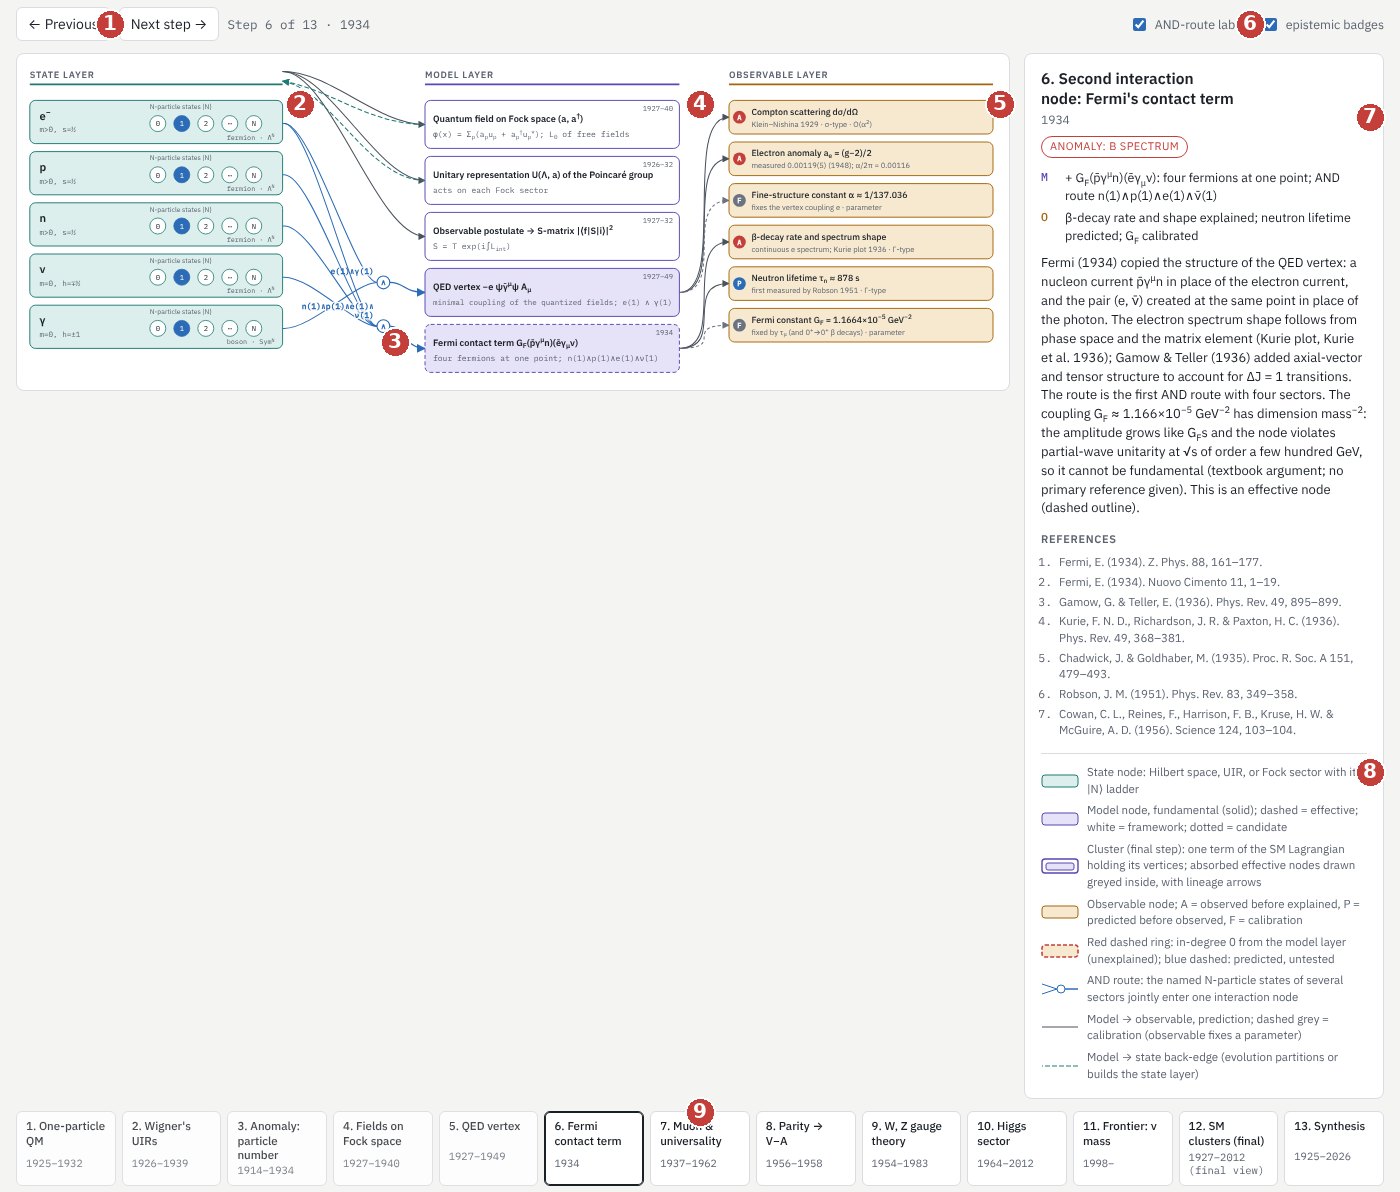
\includegraphics[width=\linewidth]{ui_annotated.png}
\caption{The page at Step 6, with its parts numbered: (1) step controls, (2) state column, (3) an AND junction, (4) model column, (5) observable column, (6) display toggles, (7) the rail with the step text and references, (8) the legend, (9) the step timeline.}\label{fig:ui}\end{figure}

\subsection{Reading one step}
\begin{enumerate}
\item \textbf{Step controls (1).} ``Next step'' and ``Previous'' move through the \nSteps{} steps; the left and right arrow keys do the same. The counter shows the step number and its years. Each step has its own address (\texttt{\#step-7}), so a step can be bookmarked or sent.
\item \textbf{State column (2).} From Step~4 on, each box is one field sector: its name, its Wigner label ($m>0$, $s=\tfrac12$, \dots), its statistics (fermion $\Lambda^N$ or boson Sym$^N$), and its occupation ladder $0,1,2,\dots,N$. A blue filled rung is an occupation number that enters a route in the current step. In Steps~1--3 the column holds the Hilbert space and the representation classes instead.
\item \textbf{AND junction (3).} Blue lines leave the rungs of several sectors and meet at a circle marked $\wedge$; one blue arrow continues into a model node. The label beside the junction names the legs, e.g.\ $n(1)\wedge p(1)\wedge e(1)\wedge\bar\nu(1)$. The toggle ``AND-route labels'' (6) hides these labels when the picture is dense.
\item \textbf{Model column (4).} Framework nodes are white; interaction nodes are violet, dashed if effective, dotted if candidate. Each node shows its years, its name and its formula. In Step~12 the nodes are grouped into clusters, one per Lagrangian term, with the absorbed effective nodes greyed inside.
\item \textbf{Observable column (5).} Each chip carries a badge (A, P or F, see the legend) and a one-line value or reference. A red dashed ring means the observable has no model edge in this step; a blue dashed ring means a prediction not yet tested.
\item \textbf{Rail (7).} The rail shows the step: title, years, the driver of the step (anomaly, symmetry, model response, prediction, clustering), what changed in each layer, the narrative, and the numbered references. \textbf{Clicking a node} replaces the rail with that node's page: formula, description, instances, its edges in this step with their relations, and its references. \textbf{Hovering an edge} highlights it and shows its mathematical relation in a tooltip; \textbf{clicking an edge} opens the relation in the rail. ``Back to step'' or the Escape key returns to the step text.
\item \textbf{Legend (8)} and \textbf{timeline (9).} The legend is repeated under every step text. The timeline at the bottom lists all steps with their years and jumps to any of them.
\item \textbf{Step 13, the method in action.} The last step replaces the graph with the synthesis: the method cycle on the left, the compact schematic on the right, and the operation log below (Figures~\ref{fig:m4}--\ref{fig:m12}). Use the numbered buttons or the arrows to choose a step, or press Play to run all twelve; hover a node in the schematic for its name, hover a phase in the cycle for its definition. Below it are the count charts and the table of changes per layer.
\end{enumerate}

\subsection{How to study the history with the page}
A productive order for a student is: read Step~1 and Step~2 for the kinematics; at Step~3 look for the red ring and ask what kind of model node could reach it before pressing ``Next''; at Step~4 click the field node and the sector boxes to see the back-edge and the ladders; from Step~5 on, for every new violet node, hover its route and its observable edges and read the relation on each edge (this is where the physics is); at Steps~8 and~9 watch the model column shrink and grow; at Step~12 open the gauge--fermion cluster and follow the lineage edges from Fermi's node to the charged current; finally read Step~13 for the counts.

\subsection{Versions}
The repository keeps every version. \texttt{v1.0/} is the first release (eleven graph steps and a synthesis), \texttt{v1.1/} adds the clustered final step, \texttt{v1.2/} adds the method-in-action synthesis view, and \texttt{latest/} always opens the newest version. Each page has a version bar at the top that links to the other versions; earlier versions show a notice pointing to the newest. The landing page lists what changed in each version.

\subsection{Data and derived files}
\begin{itemize}
\item \texttt{data/v1.2\_sm\_epistemic\_graph.json}: the full graph (nodes, references, steps with edges, routes, groups, clusters, and the phases and operations of each step), described in Appendix~\ref{app:data}. The page reads the same data embedded in its HTML.
\item \texttt{data/statistics.json}: per-step counts (nodes per layer, routes, unexplained observables).
\item \texttt{catalog.md}: every node, edge and route of every step as Markdown tables, with the references.
\item \texttt{tools/build\_derived.py}: regenerates the statistics, the catalogue, and every table and number of this paper from the JSON, so that the paper cannot drift from the graph.
\item \texttt{paper/}: this document, compiled with XeLaTeX (\texttt{latexmk -xelatex main.tex}).
\end{itemize}

\subsection{How to extend the graph}
A new node is a new entry in the \texttt{NODES} dictionary of the page (or of the JSON) with its layer, kind, label, years, description and references. A new step is a new entry in \texttt{STEPS} that lists the node identifiers of each layer, the edges with their relations, the routes with their legs, and, if the step removes nodes, the \texttt{morph} map that says which node each removed one animates into. To add the strong sector, for example, one would add the sectors $n$, $p$ (already present) and $\pi$, the Yukawa pion--nucleon node with the route $n(1)\wedge p(1)\wedge\pi(1)$, its observables (nucleon--nucleon and pion--nucleon cross sections, the deuteron), and later the quark and gluon sectors with the QCD vertex and the lineage edge that absorbs the pion node as a low-energy effective theory. After editing, \texttt{python3 tools/build\_derived.py} rebuilds the derived files, and a new version folder keeps the previous page intact. The GEN rule for edges applies: a relation the literature establishes must be an edge, so two nodes stay unconnected only when no edge can be made from the literature, and a missing edge is either a defect to report or a research target.


\section{Limitations and open edges}\label{sec:limits}
\begin{itemize}
\item \emph{Scope.} The strong sector is omitted. Adding it is a parallel branch: Yukawa's pion--nucleon node (1935), its observables (nucleon--nucleon and pion--nucleon cross sections), and its absorption not into a term that reproduces it as a low-energy limit but into QCD, where the pion is a bound state and the nucleon sectors are replaced rather than merged. That branch would test Rule~7 in a case where absorption and replacement coincide.
\item \emph{Order.} Steps~2 and~4 are in logical rather than chronological order; the page states this at Step~2.
\item \emph{Simplifications.} Antiparticles share the sector of the particle; the hadronic current is written at nucleon level until Step~9; each route is drawn from the minimal occupation numbers; colour is not drawn; neutrinos are massless until Step~11; the three-generation CKM structure is reduced to $\cos\theta_C$.
\item \emph{References.} Two references carry a note that their page numbers were not verified (Puppi 1948; Bludman 1958). The unitarity bound of the Fermi theory is quoted as a textbook argument. Numerical values are rounded PDG 2024 values~\cite{PDG2024}.
\item \emph{Open edges.} Neutrino oscillation has no established model edge (the candidate cluster is dashed); the Higgs self-coupling has a model edge and no observation. Both are research targets in the GEN sense: an edge the literature does not yet establish.
\end{itemize}

\section{Conclusion}
A three-layer concept graph with routes and badges is enough to record how particle physics was built, and the record has structure: the state layer is changed only by symmetry, by a model node's back-edge, or by an observable that distinguishes sectors; the model layer grows only against an unexplained observable or a theory-internal inconsistency; effective nodes proliferate, merge when they share a coupling, and are absorbed by fundamental nodes that reproduce them at low energy; the fundamental nodes finally cluster by Lagrangian term. These are the rules of Section~\ref{sec:laws}. They were read off one instance and are stated so that the next instance, the strong sector, can confirm or break them.

\section{AI-generation disclosure and invitation}\label{sec:ai}
The graph data, the interactive page, the scripts and the text of this paper were generated by an AI assistant (Claude, Anthropic) in conversation with the author, who specified the layers, the edge conventions, the historical order, the clustering rule and the scope, and reviewed the output. Citations were written from the assistant's knowledge and should be verified against the sources before any formal use; two are already flagged. The repository is open to community review, modification and addition: an edge that the literature establishes and the graph lacks is a defect to be reported, and an edge that the literature does not establish is a research target.

\appendix
\section{Node catalogue}\label{app:catalog}
The identifiers below are the ones used in the page's JSON data (\texttt{data/v1.2\_sm\_epistemic\_graph.json}) and in the tables of this paper. Rich markup in labels (super- and subscripts) is rendered as on the page.
\begin{longtable}{@{}l>{\raggedright\arraybackslash}p{7.6cm}lll@{}}
\caption{State-layer nodes.}\label{tab:nodesS}\\
\toprule id & label & kind & years & step\\\midrule\endfirsthead
\toprule id & label & kind & years & step\\\midrule\endhead
\bottomrule\endfoot
\texttt{H1} & H\textsubscript{1} — one-particle Hilbert space & Hilbert space & 1925–32 & 1\\
\texttt{u\_01} & m = 0, h = ±1 & UIR & 1939 & 2\\
\texttt{u\_02} & m = 0, h = ±2 & UIR & 1939 & 2\\
\texttt{u\_0h} & m = 0, h = ±½ & UIR & 1939 & 2\\
\texttt{u\_cs} & m = 0, continuous spin & UIR & 1939 & 2\\
\texttt{u\_m0} & m > 0, s = 0 & UIR & 1939 & 2\\
\texttt{u\_m1} & m > 0, s = 1 & UIR & 1939 & 2\\
\texttt{u\_mh} & m > 0, s = ½ & UIR & 1939 & 2\\
\texttt{u\_tach} & m\textsuperscript{2} < 0 & UIR & 1939 & 2\\
\texttt{u\_vac} & p\textsuperscript{μ} = 0 & UIR & 1939 & 2\\
\texttt{s\_e} & e\textsuperscript{−} & Fock sector & 1897 / field 1928 & 4\\
\texttt{s\_g} & γ & Fock sector & field 1927 & 4\\
\texttt{s\_n} & n & Fock sector & 1932 & 4\\
\texttt{s\_nu} & ν & Fock sector & 1930 / 1956 & 4\\
\texttt{s\_p} & p & Fock sector & 1919 & 4\\
\texttt{s\_mu} & μ & Fock sector & 1937 & 7\\
\texttt{s\_nue} & ν\textsubscript{e} & Fock sector & 1962 & 7\\
\texttt{s\_num} & ν\textsubscript{μ} & Fock sector & 1962 & 7\\
\texttt{s\_W} & W\textsuperscript{±} & Fock sector & 1983 & 9\\
\texttt{s\_Z} & Z\textsuperscript{0} & Fock sector & 1983 & 9\\
\texttt{s\_d} & d & Fock sector & 1964 / 1969 & 9\\
\texttt{s\_u} & u & Fock sector & 1964 / 1969 & 9\\
\texttt{s\_H} & H & Fock sector & 2012 & 10\\
\end{longtable}

\begin{longtable}{@{}l>{\raggedright\arraybackslash}p{7.6cm}lll@{}}
\caption{Model-layer nodes.}\label{tab:nodesM}\\
\toprule id & label & kind & years & step\\\midrule\endfirsthead
\toprule id & label & kind & years & step\\\midrule\endhead
\bottomrule\endfoot
\texttt{m\_A} & Observable postulate: Â = Â\textsuperscript{†}, Born rule & framework & 1927–32 & 1\\
\texttt{m\_L} & Particle Lagrangian L = ½mẋ\textsuperscript{2} − V(x) & framework & 1926 & 1\\
\texttt{m\_U} & Unitary evolution U(t) = e\textsuperscript{−iĤt/ħ} & framework & 1926–32 & 1\\
\texttt{m\_field} & Quantum field on Fock space (a, a\textsuperscript{†}) & framework & 1927–40 & 4\\
\texttt{m\_qed} & QED vertex −e ψ̄γ\textsuperscript{μ}ψ A\textsubscript{μ} & fundamental & 1927–49 & 5\\
\texttt{m\_fermi} & Fermi contact term G\textsubscript{F}(p̄γ\textsuperscript{μ}n)(ēγ\textsubscript{μ}ν) & effective & 1934 & 6\\
\texttt{m\_mu} & Muon-decay contact term (G\textsubscript{F}/√2)(ν̄\textsubscript{μ}γ\textsuperscript{μ}μ)(ēγ\textsubscript{μ}ν\textsubscript{e}) & effective & 1947–50 & 7\\
\texttt{m\_va} & Universal V−A current–current (G\textsubscript{F}/√2) J\textsubscript{μ}J\textsuperscript{μ†} & effective & 1958 & 8\\
\texttt{m\_cc} & Charged-current gauge vertex (g/√2) W\textsuperscript{+}\textsubscript{μ} J\textsuperscript{μ}\textsubscript{CC} + h.c. & fundamental & 1961–67 & 9\\
\texttt{m\_gs} & Gauge self-interactions ⊃ WWγ, WWZ, WWWW, WWZZ & fundamental & 1954 / 1961 & 9\\
\texttt{m\_nc} & Neutral-current vertex (g/cosθ\textsubscript{W}) Z\textsubscript{μ} J\textsuperscript{μ}\textsubscript{NC} & fundamental & 1961–67 & 9\\
\texttt{m\_hg} & Higgs–gauge |D\textsubscript{μ}Φ|\textsuperscript{2} → M\textsubscript{W} = gv/2, M\textsubscript{Z} = M\textsubscript{W}/cosθ\textsubscript{W} & fundamental & 1964–67 & 10\\
\texttt{m\_pot} & Higgs potential V = −μ\textsuperscript{2}Φ\textsuperscript{†}Φ + λ(Φ\textsuperscript{†}Φ)\textsuperscript{2} → m\textsubscript{H}\textsuperscript{2} = 2λv\textsuperscript{2} & fundamental & 1964 & 10\\
\texttt{m\_yuk} & Yukawa couplings −y\textsubscript{f} Φ f̄\textsubscript{L}f\textsubscript{R} + h.c. → m\textsubscript{f} = y\textsubscript{f}v/√2 & fundamental & 1967 & 10\\
\texttt{m\_numass} & Candidate: ν mass term (LΦ)(LΦ)/Λ or ν\textsubscript{R} Yukawa & candidate & 1977–79 & 11\\
\texttt{c\_bsm} & Beyond the SM: candidate ν-mass term & cluster & 1977– & 12\\
\texttt{c\_gf} & Gauge–fermion term Σ f̄ iγ\textsuperscript{μ}D\textsubscript{μ} f ⊃ EM, CC, NC vertices & cluster & 1961–67 & 12\\
\texttt{c\_gg} & Gauge kinetic term −¼W\textsuperscript{a}\textsubscript{μν}W\textsuperscript{aμν} − ¼B\textsubscript{μν}B\textsuperscript{μν} & cluster & 1954 / 1961 & 12\\
\texttt{c\_hg} & Higgs–gauge term |D\textsubscript{μ}Φ|\textsuperscript{2} & cluster & 1964–67 & 12\\
\texttt{c\_pot} & Higgs potential −V(Φ), V = −μ\textsuperscript{2}Φ\textsuperscript{†}Φ + λ(Φ\textsuperscript{†}Φ)\textsuperscript{2} & cluster & 1964 & 12\\
\texttt{c\_yuk} & Yukawa term −y\textsubscript{f} f̄\textsubscript{L}Φ f\textsubscript{R} + h.c. & cluster & 1967 & 12\\
\end{longtable}

\begin{longtable}{@{}l>{\raggedright\arraybackslash}p{7.6cm}lll@{}}
\caption{Observable-layer nodes; badge A = observed before explained, P = predicted before observed, F = calibration.}\label{tab:nodesO}\\
\toprule id & label & badge & years & step\\\midrule\endfirsthead
\toprule id & label & badge & years & step\\\midrule\endhead
\bottomrule\endfoot
\texttt{o\_E} & Energy levels (spectrum of Ĥ) & A & 1926 & 1\\
\texttt{o\_L} & Orbital angular momentum L̂\textsuperscript{2}, L̂\textsubscript{z} &  & 1926 & 1\\
\texttt{o\_S} & Spin Ŝ\textsubscript{z} = ±ħ/2 & A & 1925–27 & 1\\
\texttt{o\_p} & Momentum p̂ &  & 1926 & 1\\
\texttt{o\_x} & Position x̂ &  & 1926 & 1\\
\texttt{o\_m} & Mass m (Casimir P\textsuperscript{μ}P\textsubscript{μ} = m\textsuperscript{2}) & P & 1939 & 2\\
\texttt{o\_s} & Spin s / helicity h (Casimir W\textsuperscript{μ}W\textsubscript{μ}) & P & 1939 & 2\\
\texttt{o\_prod} & Particle production and decay & A & 1917–34 & 3\\
\texttt{o\_G} & Decay width Γ (lifetime τ = ħ/Γ) & A & 1927– & 4\\
\texttt{o\_sig} & Cross section σ, dσ/dΩ & A & 1937– & 4\\
\texttt{o\_ae} & Electron anomaly a\textsubscript{e} = (g−2)/2 & A & 1947–48 & 5\\
\texttt{o\_alpha} & Fine-structure constant α ≈ 1/137.036 & F & 1916– & 5\\
\texttt{o\_beta} & β-decay rate and spectrum shape & A & 1914 / 1934 & 5\\
\texttt{o\_compton} & Compton scattering dσ/dΩ & A & 1923 / 1929 & 5\\
\texttt{o\_lamb} & Lamb shift 2S\textsubscript{1/2} − 2P\textsubscript{1/2} & A & 1947 & 5\\
\texttt{o\_pair} & e\textsuperscript{+}e\textsuperscript{−} pair production σ(γ → e\textsuperscript{+}e\textsuperscript{−}) & P & 1932–34 & 5\\
\texttt{o\_GF} & Fermi constant G\textsubscript{F} = 1.1664×10\textsuperscript{−5} GeV\textsuperscript{−2} & F & 1934– & 6\\
\texttt{o\_ntau} & Neutron lifetime τ\textsubscript{n} ≈ 878 s & P & 1951 & 6\\
\texttt{o\_michel} & Michel spectrum, ρ = ¾ & P & 1950 & 7\\
\texttt{o\_mutau} & Muon lifetime τ\textsubscript{μ} = 2.197 μs & A & 1940– & 7\\
\texttt{o\_twonu} & ν\textsubscript{μ} ≠ ν\textsubscript{e} & P & 1962 & 7\\
\texttt{o\_hel} & Neutrino helicity h(ν) = −1 & P & 1958 & 8\\
\texttt{o\_wu} & Parity-violating asymmetries (\textsuperscript{60}Co; μ decay) & P & 1957 & 8\\
\texttt{o\_mw} & M\textsubscript{W} = 80.37 GeV & P & 1983– & 9\\
\texttt{o\_mz} & M\textsubscript{Z} = 91.19 GeV & P & 1983– & 9\\
\texttt{o\_nc} & Neutral-current events, R\textsubscript{ν} = σ(NC)/σ(CC) & P & 1973 & 9\\
\texttt{o\_nnu} & Z width → N\textsubscript{ν} = 2.984 ± 0.008 & P & 1989–2006 & 9\\
\texttt{o\_sw} & Weak mixing angle sin\textsuperscript{2}θ\textsubscript{W} ≈ 0.23 & F & 1973– & 9\\
\texttt{o\_tgc} & σ(e\textsuperscript{+}e\textsuperscript{−} → W\textsuperscript{+}W\textsuperscript{−}) and triple-gauge couplings & P & 1996–2000 & 9\\
\texttt{o\_hbr} & Higgs rates σ×BR: γγ, ZZ\textsuperscript{*}, WW\textsuperscript{*}, ττ, bb̄ & P & 2012– & 10\\
\texttt{o\_lam} & Higgs self-coupling λ\textsubscript{HHH} & P & open & 10\\
\texttt{o\_mf} & Fermion masses m\textsubscript{e}, m\textsubscript{μ}, m\textsubscript{u}, m\textsubscript{d} & F & — & 10\\
\texttt{o\_mh} & Higgs mass m\textsubscript{H} = 125.2 GeV & P & 2012 & 10\\
\texttt{o\_osc} & ν flavour oscillation: Δm\textsuperscript{2}\textsubscript{21}, Δm\textsuperscript{2}\textsubscript{31} ≠ 0 & A & 1998– & 11\\
\end{longtable}


\section{Data format}\label{app:data}
The JSON file has four parts: \texttt{conventions} (layer names, edge kinds, badge meanings, the unexplained rule); \texttt{nodes}, a dictionary from identifier to node (layer, kind, label, sub-label, years, description, instances, references, badge); \texttt{references}, a dictionary from short key to full reference; and \texttt{steps}, the ordered list of steps. A step lists its \texttt{S}, \texttt{M} and \texttt{O} node identifiers, its \texttt{edges} (from, to, kind, status, relation), its AND routes \texttt{ands} (legs as sector--occupation pairs or group--occupation pairs, target, label, relation), optional \texttt{groups} (named sets of sectors used as a single leg), optional \texttt{override} (per-step label changes), optional \texttt{morph} (which old node a removed node animates into), \texttt{phases} (the phases of the method cycle active in the step) and \texttt{ops} (the operations the step applies to the graph, each with its layer or edge kind and a description), and, for the final step, \texttt{clusters} (members and lineage edges). \texttt{tools/build\_derived.py} regenerates \texttt{data/statistics.json}, \texttt{catalog.md} and every table and macro of this paper from that file.

\begin{thebibliography}{99}
\bibitem{Heisenberg1925} Heisenberg, W. (1925). Z. Phys. 33, 879–893.
\bibitem{Schrdinger1926} Schrödinger, E. (1926). Ann. Phys. 384, 361–376 (first communication).
\bibitem{Born1926} Born, M. (1926). Z. Phys. 37, 863–867.
\bibitem{vonNeumann1932} von Neumann, J. (1932). Mathematische Grundlagen der Quantenmechanik. Springer.
\bibitem{Stone1932} Stone, M. H. (1932). Ann. Math. 33, 643–648.
\bibitem{Dirac1933} Dirac, P. A. M. (1933). Phys. Z. Sowjetunion 3, 64–72 (the Lagrangian in quantum mechanics).
\bibitem{Klein1926} Klein, O. (1926). Z. Phys. 37, 895–906.
\bibitem{Gordon1926} Gordon, W. (1926). Z. Phys. 40, 117–133.
\bibitem{Dirac1928} Dirac, P. A. M. (1928). Proc. R. Soc. A 117, 610–624.
\bibitem{Wigner1939} Wigner, E. (1939). Ann. Math. 40, 149–204.
\bibitem{BargmannandWigner1948} Bargmann, V. \& Wigner, E. P. (1948). Proc. Natl. Acad. Sci. 34, 211–223.
\bibitem{Weinberg1995} Weinberg, S. (1995). The Quantum Theory of Fields, Vol. I, ch. 2, 4, 5. Cambridge.
\bibitem{Einstein1917} Einstein, A. (1917). Phys. Z. 18, 121–128.
\bibitem{Chadwick1914} Chadwick, J. (1914). Verh. Dtsch. Phys. Ges. 16, 383–391.
\bibitem{EllisandWooster1927} Ellis, C. D. \& Wooster, W. A. (1927). Proc. R. Soc. A 117, 109–123.
\bibitem{Anderson1933} Anderson, C. D. (1933). Phys. Rev. 43, 491–494.
\bibitem{BlackettandOcchialini1933} Blackett, P. M. S. \& Occhialini, G. P. S. (1933). Proc. R. Soc. A 139, 699–726.
\bibitem{Dirac1927} Dirac, P. A. M. (1927). Proc. R. Soc. A 114, 243–265.
\bibitem{JordanandWigner1928} Jordan, P. \& Wigner, E. (1928). Z. Phys. 47, 631–651.
\bibitem{HeisenbergandPauli1929} Heisenberg, W. \& Pauli, W. (1929). Z. Phys. 56, 1–61.
\bibitem{Fock1932} Fock, V. (1932). Z. Phys. 75, 622–647.
\bibitem{Fierz1939} Fierz, M. (1939). Helv. Phys. Acta 12, 3–37.
\bibitem{Pauli1940} Pauli, W. (1940). Phys. Rev. 58, 716–722.
\bibitem{Wheeler1937} Wheeler, J. A. (1937). Phys. Rev. 52, 1107–1122.
\bibitem{Heisenberg1943} Heisenberg, W. (1943). Z. Phys. 120, 513–538.
\bibitem{Dyson1949} Dyson, F. J. (1949). Phys. Rev. 75, 486–502.
\bibitem{KleinandNishina1929} Klein, O. \& Nishina, Y. (1929). Z. Phys. 52, 853–868.
\bibitem{Dirac1931} Dirac, P. A. M. (1931). Proc. R. Soc. A 133, 60–72.
\bibitem{BetheandHeitler1934} Bethe, H. \& Heitler, W. (1934). Proc. R. Soc. A 146, 83–112.
\bibitem{LambandRetherford1947} Lamb, W. E. \& Retherford, R. C. (1947). Phys. Rev. 72, 241–243.
\bibitem{Bethe1947} Bethe, H. A. (1947). Phys. Rev. 72, 339–341.
\bibitem{KuschandFoley1948} Kusch, P. \& Foley, H. M. (1948). Phys. Rev. 74, 250–263.
\bibitem{Schwinger1948} Schwinger, J. (1948). Phys. Rev. 73, 416–417.
\bibitem{Tomonaga1946} Tomonaga, S. (1946). Prog. Theor. Phys. 1, 27–42.
\bibitem{Feynman1949} Feynman, R. P. (1949). Phys. Rev. 76, 769–789.
\bibitem{Fermi1934a} Fermi, E. (1934). Z. Phys. 88, 161–177.
\bibitem{Fermi1934b} Fermi, E. (1934). Nuovo Cimento 11, 1–19.
\bibitem{GamowandTeller1936} Gamow, G. \& Teller, E. (1936). Phys. Rev. 49, 895–899.
\bibitem{Kurieetal1936} Kurie, F. N. D., Richardson, J. R. \& Paxton, H. C. (1936). Phys. Rev. 49, 368–381.
\bibitem{ChadwickandGoldhaber1935} Chadwick, J. \& Goldhaber, M. (1935). Proc. R. Soc. A 151, 479–493.
\bibitem{Robson1951} Robson, J. M. (1951). Phys. Rev. 83, 349–358.
\bibitem{Cowanetal1956} Cowan, C. L., Reines, F., Harrison, F. B., Kruse, H. W. \& McGuire, A. D. (1956). Science 124, 103–104.
\bibitem{Chadwick1932} Chadwick, J. (1932). Proc. R. Soc. A 136, 692–708.
\bibitem{NeddermeyerandAnderson1937} Neddermeyer, S. H. \& Anderson, C. D. (1937). Phys. Rev. 51, 884–886.
\bibitem{Conversietal1947} Conversi, M., Pancini, E. \& Piccioni, O. (1947). Phys. Rev. 71, 209–210.
\bibitem{Puppi1948} Puppi, G. (1948). Nuovo Cimento 5, 587–588. \textit{[page numbers to be verified]}
\bibitem{Klein1948} Klein, O. (1948). Nature 161, 897–899.
\bibitem{TiomnoandWheeler1949} Tiomno, J. \& Wheeler, J. A. (1949). Rev. Mod. Phys. 21, 144–152.
\bibitem{LeeRosenbluthandYang1949} Lee, T. D., Rosenbluth, M. \& Yang, C. N. (1949). Phys. Rev. 75, 905.
\bibitem{Michel1950} Michel, L. (1950). Proc. Phys. Soc. A 63, 514–531.
\bibitem{Danbyetal1962} Danby, G. et al. (1962). Phys. Rev. Lett. 9, 36–44.
\bibitem{LeeandYang1956} Lee, T. D. \& Yang, C. N. (1956). Phys. Rev. 104, 254–258.
\bibitem{Wuetal1957} Wu, C. S., Ambler, E., Hayward, R. W., Hoppes, D. D. \& Hudson, R. P. (1957). Phys. Rev. 105, 1413–1415.
\bibitem{Garwinetal1957} Garwin, R. L., Lederman, L. M. \& Weinrich, M. (1957). Phys. Rev. 105, 1415–1417.
\bibitem{FeynmanandGellMann1958} Feynman, R. P. \& Gell-Mann, M. (1958). Phys. Rev. 109, 193–198.
\bibitem{SudarshanandMarshak1958} Sudarshan, E. C. G. \& Marshak, R. E. (1958). Phys. Rev. 109, 1860–1862.
\bibitem{Goldhaberetal1958} Goldhaber, M., Grodzins, L. \& Sunyar, A. W. (1958). Phys. Rev. 109, 1015–1017.
\bibitem{Cabibbo1963} Cabibbo, N. (1963). Phys. Rev. Lett. 10, 531–533.
\bibitem{YangandMills1954} Yang, C. N. \& Mills, R. L. (1954). Phys. Rev. 96, 191–195.
\bibitem{Schwinger1957} Schwinger, J. (1957). Ann. Phys. 2, 407–434.
\bibitem{Bludman1958} Bludman, S. A. (1958). Nuovo Cimento 9, 433–445. \textit{[page numbers to be verified]}
\bibitem{Glashow1961} Glashow, S. L. (1961). Nucl. Phys. 22, 579–588.
\bibitem{Weinberg1967} Weinberg, S. (1967). Phys. Rev. Lett. 19, 1264–1266.
\bibitem{Salam1968} Salam, A. (1968). In Elementary Particle Theory (Nobel Symp. 8), ed. N. Svartholm, 367–377. Almqvist \& Wiksell.
\bibitem{tHooft1971} 't Hooft, G. (1971). Nucl. Phys. B 35, 167–188.
\bibitem{tHooftandVeltman1972} 't Hooft, G. \& Veltman, M. (1972). Nucl. Phys. B 44, 189–213.
\bibitem{Hasertetal1973} Hasert, F. J. et al. (1973). Phys. Lett. B 46, 138–140.
\bibitem{Arnisonetal1983} Arnison, G. et al. (UA1) (1983). Phys. Lett. B 122, 103–116.
\bibitem{Banneretal1983} Banner, M. et al. (UA2) (1983). Phys. Lett. B 122, 476–485.
\bibitem{Arnisonetal1983b} Arnison, G. et al. (UA1) (1983). Phys. Lett. B 126, 398–410.
\bibitem{LEPEWWG2006} ALEPH, DELPHI, L3, OPAL, SLD, LEP EWWG, SLD EW \& HF groups (2006). Phys. Rep. 427, 257–454.
\bibitem{LEP2EWWG2013} ALEPH, DELPHI, L3, OPAL, LEP EWWG (2013). Phys. Rep. 532, 119–244.
\bibitem{GellMann1964} Gell-Mann, M. (1964). Phys. Lett. 8, 214–215.
\bibitem{Bloometal1969} Bloom, E. D. et al. (1969). Phys. Rev. Lett. 23, 930–934.
\bibitem{Weinberg1979} Weinberg, S. (1979). Physica A 96, 327–340 (phenomenological Lagrangians).
\bibitem{Weinberg1979b} Weinberg, S. (1979). Phys. Rev. Lett. 43, 1566–1570.
\bibitem{EnglertandBrout1964} Englert, F. \& Brout, R. (1964). Phys. Rev. Lett. 13, 321–323.
\bibitem{Higgs1964} Higgs, P. W. (1964). Phys. Rev. Lett. 13, 508–509.
\bibitem{GuralnikHagenandKibble1964} Guralnik, G. S., Hagen, C. R. \& Kibble, T. W. B. (1964). Phys. Rev. Lett. 13, 585–587.
\bibitem{ATLAS2012} ATLAS Collaboration (2012). Phys. Lett. B 716, 1–29.
\bibitem{CMS2012} CMS Collaboration (2012). Phys. Lett. B 716, 30–61.
\bibitem{Fukudaetal1998} Fukuda, Y. et al. (Super-Kamiokande) (1998). Phys. Rev. Lett. 81, 1562–1567.
\bibitem{Ahmadetal2002} Ahmad, Q. R. et al. (SNO) (2002). Phys. Rev. Lett. 89, 011301.
\bibitem{Eguchietal2003} Eguchi, K. et al. (KamLAND) (2003). Phys. Rev. Lett. 90, 021802.
\bibitem{Minkowski1977} Minkowski, P. (1977). Phys. Lett. B 67, 421–428.
\bibitem{MohapatraandSenjanovi1980} Mohapatra, R. N. \& Senjanović, G. (1980). Phys. Rev. Lett. 44, 912–915.
\bibitem{PDG2024} Particle Data Group, Navas, S. et al. (2024). Phys. Rev. D 110, 030001.
\end{thebibliography}

\end{document}
